%% ----------------------------------------------------------------
%% Project.tex
%% ----------------------------------------------------------------
\documentclass[openany]{ecsproject}     % Use the Project Style
\graphicspath{{images/}}   % Location of your graphics files
%\DeclareGraphicsExtensions{.png, .jpg, .eps}
\usepackage{pdfpages}
\usepackage[titletoc]{appendix}
\usepackage[square,numbers]{natbib}            % Use Natbib style for the refs.
\hypersetup{colorlinks=true}   % Set to false for black/white printing
%% ----------------------------------------------------------------
%% Definitions.tex
%% ---------------------------------------------------------------- 
\newcommand{\BibTeX}{{\rm B\kern-.05em{\sc i\kern-.025em b}\kern-.08em T\kern-.1667em\lower.7ex\hbox{E}\kern-.125emX}}

%% People
\newcounter{address}
\setcounter{address}{1}
\renewcommand{\theaddress}{\textsuperscript{\fnsymbol{address}}}
\newcommand{\address}[1]{\refstepcounter{address}\theaddress#1\\}
\newcommand{\Name}[3]{\texorpdfstring{\href{mailto:#3}{#2}#1}{#2}\xspace}
\newcommand{\SteveRGunn}[1]{\Name{#1}{Steve R. Gunn}{S.R.Gunn@ecs.soton.ac.uk}}

%% Dingbats
\newcommand{\tick}{\ding{51}}
\newcommand{\cross}{\ding{55}}

%% Calculus
\newcommand{\pd}[2]{\ensuremath{\frac{\partial #1}{\partial #2}}\xspace}
\newcommand{\fd}[2]{\ensuremath{\frac{d #1}{d #2}}\xspace}
\newcommand{\dint}{\ensuremath{\int\!\!\!\int}\xspace}
\newcommand{\tint}{\ensuremath{\int\!\!\!\int\!\!\!\int}\xspace}

%% Math Sets
\newcommand{\Q}[1]{\ensuremath{\mathbb{#1}}\xspace}
\newcommand{\R}{\Q{R}}

%% Matrix, Vector
\newcommand{\V}[1]{\ensuremath{\boldsymbol{#1}}\xspace}
\newcommand{\M}[1]{\ensuremath{\boldsymbol{#1}}\xspace}
\newcommand{\0}{\V{0}}
\newcommand{\1}{\V{1}}
\newcommand{\I}{\M{I}}

%% Math Functions
\newcommand{\F}[1]{\ensuremath{\mathrm{#1}}\xspace}
\newcommand{\sgn}{\F{sgn}}
\newcommand{\tr}{\F{trace}}
\newcommand{\diag}{\F{diag}}

%% Math Names
\newcommand{\N}[1]{\ensuremath{\mathit{#1}}\xspace}

%% Data
\newcommand{\mc}[1]{\ensuremath{\mathcal{#1}}\xspace}
\newcommand{\Hyp}{\mc{H}}
\newcommand{\D}{\mc{D}}

%% Kernel
\newcommand{\K}{\M{K}}
\newcommand{\eins}{\texorpdfstring{\ensuremath{\epsilon}}{\textepsilon}-insensitive\xspace}
\newcommand{\e}{\ensuremath{\epsilon}\xspace}
\newcommand{\Bxi}{\ensuremath{\boldsymbol{\xi}}\xspace}
\newcommand{\Kanova}{\ensuremath{\mathit{K_{ANOVA}}}\xspace}
\newcommand{\Kspline}{\ensuremath{\mathit{K_{spline}}}\xspace}

%% Bayesian
\newcommand{\MP}{\ensuremath{\mathit{{\scriptscriptstyle \hspace{-1.5pt}M\hspace{-1.5pt}P}}}\xspace}
\newcommand{\ML}{\ensuremath{\mathit{{\scriptscriptstyle \hspace{-1.5pt}M\hspace{-1.5pt}L}}}\xspace}
\newcommand{\Qw}{\ensuremath{Q_{\w}(\w)}\xspace}
\newcommand{\Qa}{\ensuremath{Q_{\Ba}(\Ba)}\xspace}
\newcommand{\Qb}{\ensuremath{Q_{\beta}(\beta)}\xspace}
\newcommand{\wMPab}{\ensuremath{\w_{\MP|\bar {\Ba},\bar \beta}}\xspace}
\newcommand{\wMP}{\ensuremath{\w_{\MP}}\xspace}
\newcommand{\yMP}{\ensuremath{y_{\MP}}\xspace}
\newcommand{\BaMP}{\ensuremath{\Ba_{\hspace{1pt}\MP}}\xspace}
\newcommand{\aMP}{\ensuremath{\alpha_{\hspace{1pt}\MP}}\xspace}
\newcommand{\bMP}{\ensuremath{\beta_{\hspace{1pt}\MP}}\xspace}
\newcommand{\Sab}{\ensuremath{\M{\Sigma}_{\bar \Ba,\bar \beta}}\xspace}
\newcommand{\Ba}{\ensuremath{\boldsymbol{\alpha}}\xspace}
\newcommand{\Bb}{\ensuremath{\boldsymbol{\beta}}\xspace}
\newcommand{\Bm}{\ensuremath{\boldsymbol{\mu}}\xspace}
\newcommand{\BL}{\ensuremath{\boldsymbol{\Lambda}}\xspace}
\newcommand{\BPhi}{\ensuremath{\boldsymbol{\Phi}}\xspace}
\newcommand{\SMP}{\ensuremath{\M{\Sigma}_{\MP}}\xspace}

\newcommand{\Pa}{\ensuremath{P(\alpha|\mathcal{H})}\xspace}
\newcommand{\Pb}{\ensuremath{P(\beta|\mathcal{H})}\xspace}
\newcommand{\Pab}{\ensuremath{P(\alpha,\beta|\mathcal{H})}\xspace}
\newcommand{\Pw}{\ensuremath{P(\w|\mathcal{H})}\xspace}
\newcommand{\PD}{\ensuremath{P(\D|\mathcal{H})}\xspace}
\newcommand{\PwIa}{\ensuremath{P(\w|\alpha,\mathcal{H})}\xspace}
\newcommand{\PDIwb}{\ensuremath{P(\D|\w,\beta,\mathcal{H})}\xspace}
\newcommand{\PDwab}{\ensuremath{P(\D,\w,\alpha,\beta|\mathcal{H})}\xspace}
\newcommand{\PDIw}{\ensuremath{P(\D|\w,\mathcal{H})}\xspace}
\newcommand{\PwID}{\ensuremath{P(\w|\D,\mathcal{H})}\xspace}
\newcommand{\PwabID}{\ensuremath{P(\w,\alpha,\beta|\D,\mathcal{H})}\xspace}

\newcommand{\PanH}{\ensuremath{P(\alpha)}\xspace}
\newcommand{\PbnH}{\ensuremath{P(\beta)}\xspace}
\newcommand{\PabnH}{\ensuremath{P(\alpha,\beta)}\xspace}
\newcommand{\PwnH}{\ensuremath{P(\w)}\xspace}
\newcommand{\PDnH}{\ensuremath{P(\D)}\xspace}
\newcommand{\PwIanH}{\ensuremath{P(\w|\alpha)}\xspace}
\newcommand{\PDIwbnH}{\ensuremath{P(\D|\w,\beta)}\xspace}
\newcommand{\PDwabnH}{\ensuremath{P(\D,\w,\Ba,\beta)}\xspace}
\newcommand{\PDIwnH}{\ensuremath{P(\D|\w)}\xspace}
\newcommand{\PwIDnH}{\ensuremath{P(\w|\D)}\xspace}
\newcommand{\PwabIDnH}{\ensuremath{P(\w,\alpha,\beta|\D)}\xspace}

\newcommand{\PDwBab}{\ensuremath{P(\D,\w,\Ba,\beta|\mathcal{H})}\xspace}
\newcommand{\PwIBa}{\ensuremath{P(\w|\Ba,\mathcal{H})}\xspace}
\newcommand{\PBab}{\ensuremath{P(\Ba,\beta|\mathcal{H})}\xspace}
\newcommand{\PwBabID}{\ensuremath{P(\w,\Ba,\beta|\D,\mathcal{H})}\xspace}

\newcommand{\PBanH}{\ensuremath{P(\Ba)}\xspace}
\newcommand{\PwIBanH}{\ensuremath{P(\w|\Ba)}\xspace}

%% Snakes
\newcommand{\Esnake}{\ensuremath{\mathit{E_{snake}}}\xspace}
\newcommand{\Eimage}{\ensuremath{\mathit{E_{image}}}\xspace}
\newcommand{\Econt}{\ensuremath{\mathit{E_{cont}}}\xspace}
\newcommand{\Ecurv}{\ensuremath{\mathit{E_{curv}}}\xspace}
\newcommand{\Eint}{\ensuremath{\mathit{E_{int}}}\xspace}
\newcommand{\Eext}{\ensuremath{\mathit{E_{ext}}}\xspace}
\newcommand{\Eterm}{\ensuremath{\mathit{E_{term}}}\xspace}
\newcommand{\Eline}{\ensuremath{\mathit{E_{line}}}\xspace}
\newcommand{\Eedge}{\ensuremath{\mathit{E_{edge}}}\xspace}
\newcommand{\Econ}{\ensuremath{\mathit{E_{con}}}\xspace}
\newcommand{\Eangle}{\ensuremath{\mathit{E_{angle}}}\xspace}
\newcommand{\Elshape}{\ensuremath{\mathit{E_{lshape}}}\xspace}
\newcommand{\Eedgedir}{\ensuremath{\mathit{E_{edgedir}}}\xspace}
\newcommand{\Emodel}{\ensuremath{\mathit{E_{model}}}\xspace}
\newcommand{\wte}{\ensuremath{\mathit{w_{term}}}\xspace}
\newcommand{\wli}{\ensuremath{\mathit{w_{line}}}\xspace}
\newcommand{\wed}{\ensuremath{\mathit{w_{edge}}}\xspace}
\newcommand{\wco}{\ensuremath{\mathit{w_{con}}}\xspace}

%% Environments
\newcounter{alg}
\newenvironment{algorithm}[1]
{
    \stepcounter{alg}
    \begin{table}[htb]
    \centering
    \begin{tabular}[t]{ll}
    \hline&\\
    \multicolumn{2}{l}{\bf Algorithm \arabic{alg}: #1}\\&\\
} {
    &\\
    \hline
    \end{tabular}
    \end{table}
}
            % Include your abbreviations
%\bibliographystyle{ecs}
\bibliographystyle{ieeetr}
\renewcommand{\bibname}{References}
%% ----------------------------------------------------------------
\begin{document}
\frontmatter
\title      {Energy Efficient Object Detection and Tracking through Adaptive Operation on Heterogeneous Multi-core Systems}
\authors    {\texorpdfstring
             {\href{mailto:yz39g13@soton.ac.uk}{Yubo Zhi}}
             {Yubo Zhi}
            }
\addresses  {\groupname\\\deptname\\\univname}
\date       {\today}
\subject    {}
\keywords   {}
\supervisor {\texorpdfstring
             {\href{mailto:gvm@ecs.soton.ac.uk}{Dr Geoff Merrett}}
             {Dr Geoff Merrett}
	    }
\examiner   {\texorpdfstring
             {\href{mailto:dan@ecs.soton.ac.uk}{Denis A Nicole}}
	     {Denis A Nicole}
	    }
\degree     {BEng Electronic Engineering}
\maketitle

\begin{abstract}
Object detection and tracking is a key technique used in computer vision applications, especially robotic systems, artificial intelligence and video surveillance systems, but video processing algorithms require a lot of computations, consume a significant amount of energy. This project is purposed to reduce power consumption and improves performance of camera based real-time object detection and tracking applications. Such an application may rely heavily on battery power or harvesting energy from environment, hence power consumption on those devices becomes critical. As battery technology development is not as fast as electronic processing technology development, lower power consumption implies longer battery life for mobile devices e.g. laptops and smart phones, also lower environmental impact.

This project investigated some hardware based approaches to achieve an overall reduction of computations required for doing continuous real-time object detection and tracking, through adaptive control of frame rate and resolution, based on whether objects detected, their location and moving speed projected onto the camera sensor.
\end{abstract}

\tableofcontents
%\listoffigures
%\listoftables
%\lstlistoflistings
%\listofsymbols{ll}{$w$ & The weight vector}

%\acknowledgements{Thanks to no one.}
%\dedicatory{To \dots}
\mainmatter

%% ----------------------------------------------------------------
\chapter{Introduction} \label{Chapter:Introduction}

\iffalse
1-1.5 pages
\fi

\section{The problem}

\iffalse
% Current energy wasting part.
% Use heterogeneous hardware.
% Needs for energy efficient object detection:
% Embedded devices, robots, etc.
% Less computation, can achieve less storage \& bandwidth.
\fi

Computer vision algorithms are heavily used in lots of different areas, such as robotic and video surveillance systems. Currently most of them requires the use of a dedicated processing server, either a remote computer or a cloud server on the internet, wasting a lot of energy and data bandwidth in the process of video stream transmission, storage and processing, also suffers high response latency. With the rapid growth of integrated circuit technologies, processing power was just enough to realise computation intensive computer vision algorithms on a small form factor mobile platform, which can be very useful for those systems, since it can dramatically reduce the energy wasting by applying computer vision algorithms directly on board, enables low latency reactions and adaptive energy saving operation, also provides considerable flexibility.

Moreover, with the availability of integrated GPU cores in modern embedded and system-on-chip (SoC) platforms, on board video processing can be a lot more faster and powerful by utilising the heterogeneous hardware architecture, as most of video processing algorithms can take the advantages of parallel computing.

%However, mobile devices generally have limited processing power, memory, storage and energy, but video processing algorithms involves lots of computations, hence could be the most power intensive and time consuming part in such application.

\section{Example applications} %\label{Chapter:Applications}

\iffalse
Example applications, can be multiple.
e.g. Video conference.
\fi

This technique can be applied to vision based robotic and interactive embedded applications, where power consumption and response latency are essential. By enabling adaptive frame rate and resolution control, the processing power, hence the total power consumption, can be dramatically reduced by not having to continuously process video stream at high frame rate and resolution when it is not necessary. In addition, by executing computer vision algorithms on board instead of remote compute server, low latency responsiveness on such system can be achieved.

This technique may also be applied to bandwidth efficient video streaming applications, for example video surveillance and conferencing. In such applications, the bandwidth and storage requirements can be significantly reduced when no noticeable object in the scene was moving, since high frame rate video streaming and storing are not necessary and can even be paused.

\section{Aims}

\iffalse
Metric: power consumption vs accuracy?
What have done?
\fi

\iffalse
The aim of this project was to investigate ways to reduce overall power consumption of camera based real-time object detection and tracking applications, by applying feedback control of the camera module based on previous tracking results and utilising existing camera hardware capabilities including down sampling and cropping instead of software algorithms, while keeping a sensible accuracy. By doing so the average computation time would be dramatically reduced, hence reducing the overall power consumption.
\fi

The targets to be achieved are:

\begin{itemize}
	\item Choose an embedded development platform that is capable for running computer vision algorithms in real time and has direct access to camera control interface.
	\item Interface a suitable camera module with sensible specifications for use with the platform.
	\item Identity and realise real time object detection and tracking algorithms that are suitable for use in such platform.
	\item Realise adaptive camera frame rate and resolution control, based on the speeds and sizes of objects tracked, hence reducing computations, consequently reducing total power consumption.
	\item Analyse and optimise the performance of the operation metric, by applying the algorithms with and without adaptive operation on same sets of sample video streams, comparing the percentage of objects been tracked and overall power consumption reduction achieved.
\end{itemize}

\iffalse
\begin{itemize}
  \item Development of a basic object tracking system, identify algorithms suitable for real-time operation, minimise operating system overheads.
  \item Interfacing camera module with the embedded system, expose control functions.
  \item Develop and analyse automatic camera frame rate reduction.
  \item Develop and analyse hardware down sampling and cropping.
  \item If time allows, object recognition may be implemented.
\end{itemize}
\fi

%\section{Example applications} %\label{Chapter:Applications}

\iffalse
Example applications, can be multiple.
e.g. Video conference.
\fi

This technique can be applied to vision based robotic and interactive embedded systems, where power consumption and reaction latency are essential. By enabling adaptive frame rate and resolution control, the processing power hence the total power consumption can be dramatically reduced, by not having to continuously process video stream at high frame rate and resolution when it is not necessary. In addition, by executing some of computer vision algorithms on board instead of remote compute server, low latency reactions on such system can be achieved.

This technique may also be applied to bandwidth efficient video streaming applications, for example video surveillance and conferencing. In such applications, .

\chapter{Background and literature search}

There are lots of different algorithms and approaches existing in the field of object detection and tracking. Some of those algorithms were investigated in this project in order to identify a set of suitable algorithms that were both accurate and efficient enough to \moda{analyse} video stream from \mdc{a camera} by an embedded platform in real time.

Object tracking typically consists of 2 steps. Initially, locations and shapes of each moving object appeared in each frame need to be identified. Subsequently, by analysing and recording the movements of each object in sequential frames, the objects in a video stream can be tracked.

\section{OpenCV computer vision library}

% {\color{red}Information...}

OpenCV computer vision library \cite{opencv} is a very powerful open-source computer vision library. \moda{It contains lots of useful computer vision algorithms designed for computational efficiency and real-time applications. It is also mostly platform independent \mdc{enabling} easy platform adaptation. Furthermore, it can take the advantage of multi-core and GPU parallel processing on heterogeneous platforms by using a dedicated GPU algorithm module.}

\section{Model based object detection algorithms}

\iffalse
Being able to detect objects in a video frame is the first, also the most important and challenging step to do object tracking. This is generally accomplished by separation of foreground objects and background image.
\fi

Object detection is generally accomplished by separation of foreground and background masks, called background subtraction or foreground segmentation.

\subsection{Colour based}
\label{bgs:colour}

\mdc{Colours} can sometimes provide enough information about a specific object, \mdc{such as} a coloured ball. For filtering a specific colour out from a video frame, hue-saturation-value (HSV) colour space \cite[p.~301]{colourspace} representation is usually used, which can make colour filtering a lot easier based on hue, saturation and brightness information of the specific colour. In this way, a foreground mask can be generated easily by filtering \mdc{the} target colour. For example, \fref{Figure:MOTBOC} shows a simple colour filtering object detection implementation \cite{MOTBOC.git} that is able to detect objects with specific colours.

\begin{figure}[H]
  \centering
  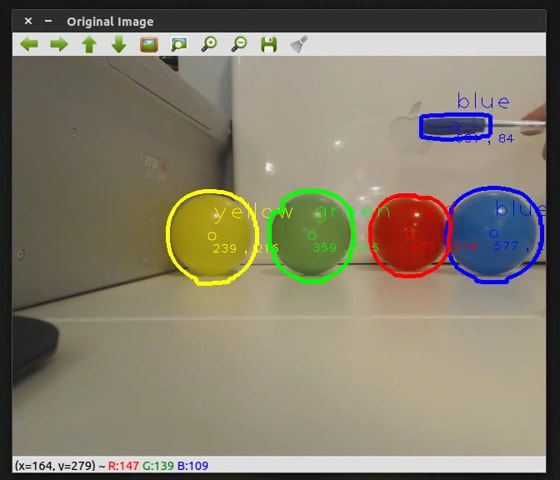
\includegraphics[width=0.5\columnwidth]{MOTBOC}
  \caption{Multi object tracking based on colour filtering (sourced from \cite{MOTBOC.git}).}
  \label{Figure:MOTBOC}
\end{figure}

This implementation does not require a lot of graphic processing, thus can be very quick and efficient, suitable for robots that are tracking something like a coloured ball or \mdc{a} piece of paper, \mdc{it} also could be useful for line racing car projects.

There are also researches using a more complex particle filtering algorithm based on colour distributions over a region in the frame \cite{nummiaro2003color}\mdc{. The results are shown in} \fref{Figure:nummiaro2003color}. \mdc{Firstly the cameras need to be calibrated and compensated. Then} a colour distribution model of the target object \mdc{needs} to be built\mdc{. Followed by that,} the elliptical region of the tracked object get determined by \mdc{applying} colour-based particle filters \cite{nummiaro2003adaptive}. The algorithm from the research are purposed to be used in multi-camera environments to select the best view of the target, therefore several views from different \mdc{cameras} are shown by the images at the bottom, along with the coefficients \mdc{implying the} similarity with the target model shown at the top left, and the selected best view at the top right.
% {\color{red}Details on algorithm implementation required.}

\begin{figure}[H]
  \centering
  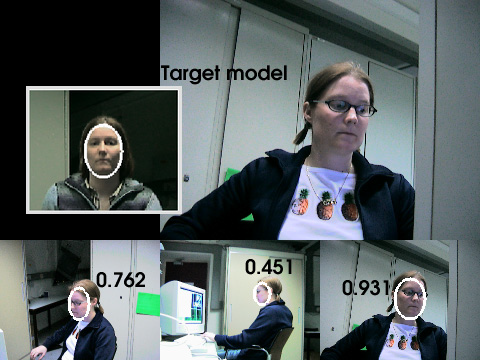
\includegraphics[width=0.5\columnwidth]{nummiaro2003color}
  \caption{Object tracking based on colour distribution particle filtering in multi-camera environments (sourced from \cite{nummiaro2003color}).}
  \label{Figure:nummiaro2003color}
\end{figure}

However, if there were other targets with \mdc{a} similar colour distribution, the algorithm \modc{might fail} to distinguish them, as shown \mdc{in} the second image in \fref{Figure:nummiaro2003color_fail}, the face of the man got tracked instead of the target woman's face. It also requires a specific model associated with each of the objects to be tracked.

\begin{figure}[H]
  \centering
  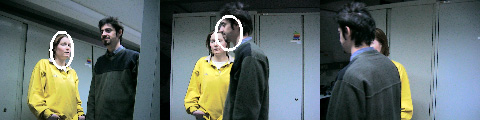
\includegraphics[width=0.9\columnwidth]{nummiaro2003color_fail}
  \caption{Problems on colour based object tracking, when several good candidates exists at the same time (sourced from \cite{nummiaro2003color}).}
  \label{Figure:nummiaro2003color_fail}
\end{figure}

\subsection{Shape matching}

Another important information about an object might be its distinctive shape. By extracting object edges in the scene \modc{and} apply appropriate shape matching algorithms, an object can be detected based on its shape.

This research \cite{borovicka2003circle} shows the ability to detect circles in a image by applying edge filtering followed by Hough \moda{transform}, as shown \mdc{in} \fref{Figure:circles}. \fref{Figure:circle:original} shows the original grey scaled image, then after blurred and Sobel filtered (\fref{Figure:circle:sobel}), clear edges \mdc{can be} extracted (\fref{Figure:circle:edge}). Finally, Hough transform \mdc{is} applied, the results merged with the original image are shown \mdc{in} \fref{Figure:circle:circles}.

\begin{figure}[H]
  \centering
  \subfigure [] {
    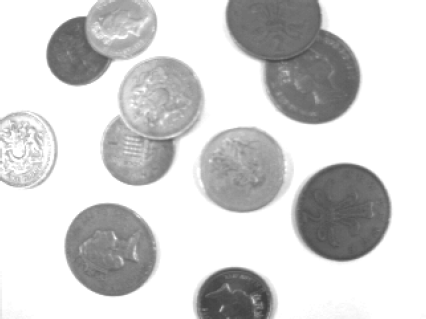
\includegraphics[width=0.22\columnwidth]{circle_original}
    \label{Figure:circle:original}
  }
  \subfigure [] {
    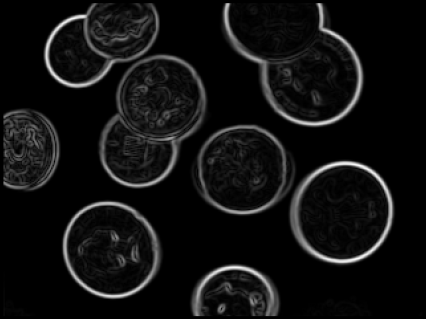
\includegraphics[width=0.22\columnwidth]{circle_sobel}
    \label{Figure:circle:sobel}
  }
  \subfigure [] {
    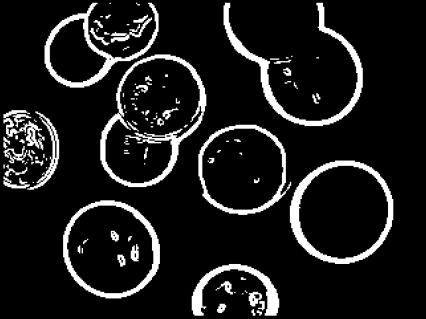
\includegraphics[width=0.22\columnwidth]{circle_edge}
    \label{Figure:circle:edge}
  }
  \subfigure [] {
    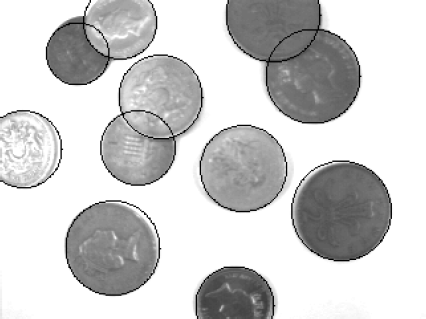
\includegraphics[width=0.22\columnwidth]{circle_circles}
    \label{Figure:circle:circles}
  }
  \caption{Circle detection by Hough transform (sourced from \cite{borovicka2003circle}). \subref{Figure:circle:original} shows the original image, \subref{Figure:circle:sobel} Sobel filters applied, \subref{Figure:circle:edge} threshold edge map, \subref{Figure:circle:circles} detected circles}
  \label{Figure:bg_circles}
\end{figure}

This implementation might be suitable for ball tracking \mdc{purposes}. By combining with the colour filtering as described in Section \ref{bgs:colour}, a single coloured ball could be efficiently tracked.

\subsection{Feature detection (Cascade classifier)}
\label{sec:bg:cc}

% {\color{red}Use this: \cite{viola2001rapid}}

Cascade classifier \cite{cascade} \cite{viola2001rapid} is a widely used object detection technique based on machine learning. By concatenating a large number of simple feature detectors (i.e. classifiers) each detecting different simple features based on \mdc{the} intensity at different positions as shown \mdc{in} \fref{bg:cc}, complex objects such as human faces can be recognised as shown in \moda{\fref{bg:cc:faces}}. Furthermore\mdc{,} its accuracy can be improved by training the classifier both positively and negatively.

\begin{figure}[H]
  \centering
  \subfigure [] {
    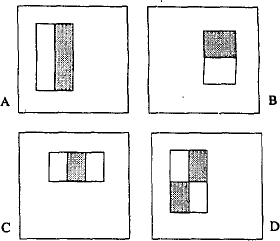
\includegraphics[width=0.3\columnwidth]{cc_features}
    \label{bg:cc:features}
  }
  \subfigure [] {
    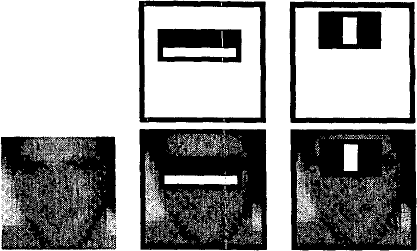
\includegraphics[width=0.3\columnwidth]{cc_face}
    \label{bg:cc:face}
  }
  \caption{Cascade classifier (sourced from \cite{borovicka2003circle}). \subref{bg:cc:features} shows some example simple feature detector configurations, \subref{bg:cc:face} shows some feature detector used on face recognition.}
  \label{bg:cc}
\end{figure}

\begin{figure}[H]
  \centering
  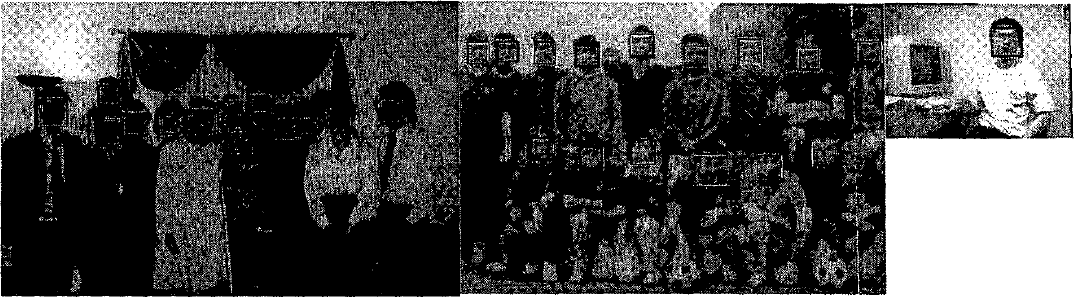
\includegraphics[width=0.9\columnwidth]{cc_faces}
  \caption{Cascade classifier recognising human faces (sourced from \cite{borovicka2003circle}).}
  \label{bg:cc:faces}
\end{figure}

This algorithm is mostly used for object classification, \mdc{such as} recognising human faces, bodies and different classes of vehicles in images. Like other \mdc{model-based} algorithms, multiple classifier definitions are required for detecting different kinds of objects, or even different perspectives of the same object.

% {\color{red}Replace with results from research paper}

\section{Motion-based object detection algorithms}

\subsection{Background subtraction}
\label{motion_bs}

By studying frames from a video stream then \mdc{building} up a background model image, it is also possible to detect moving objects in following frames efficiently.

% {\color{red}Add some graph from research paper?}

% {\color{red}Should be in design section?

% This type of algorithms suit well for static camera movement tracking, and were not limited by objects' geometry shapes, therefore was used in this project.}

% {\color{cyan}Background subtraction algorithms:

There are several background subtraction algorithms available, the BGSLibrary \cite{bgslibrary} is specifically developed for \mdc{analysing} those algorithms, it offers 37 different background subtraction algorithms implemented \mdc{by} OpenCV, published under GNU GPL v3 license. With the same programming interface for all available algorithms, it allows easy swapping between algorithms.

There is an article \cite{bgs:article} reviewed the algorithms available in the BGSLibrary, ranked \mdc{top 5 algorithms} in overall performance score as shown in \tref{Table:bgs}. \fref{bgsreview} shows foreground masks obtained from the top 5 algorithms on sequences from real world videos at the same frame. \moda{TP pixels indicate foreground pixels classified as foreground, and TN pixels indicate background pixels classified as background. Both TP and TN pixels combined \mdc{together} are the expected results, named ground truth foreground masks. FP pixels indicate background pixels classified as foreground, and FN pixels indicate foreground pixels classified as background. Both FP and FN pixels are incorrect results produced by the algorithm.} The actual foreground masks generated by the algorithms are TP and FN pixels.

\begin{table}[H]
  \centering
  \begin{tabular}{cc}
  \toprule
  \textbf{Method ID} & \textbf{Method name}\\
  \midrule
  PBAS & Pixel-Based Adaptive Segmenter \\
  MultiLayerBGS & Multi-Layer BGS \\
  MixtureOfGaussianV1BGS & Gaussian Mixture Model \\
  LBAdaptiveSOM & Adaptive SOM \\
  DPWrenGABGS & Gaussian Average \\
  \bottomrule
  \end{tabular}
  \caption{Background substraction algorithms investigated (adapted from \cite{bgslibrary})}
  \label{Table:bgs}
\end{table}

\begin{figure}[tbh]
  \centering
  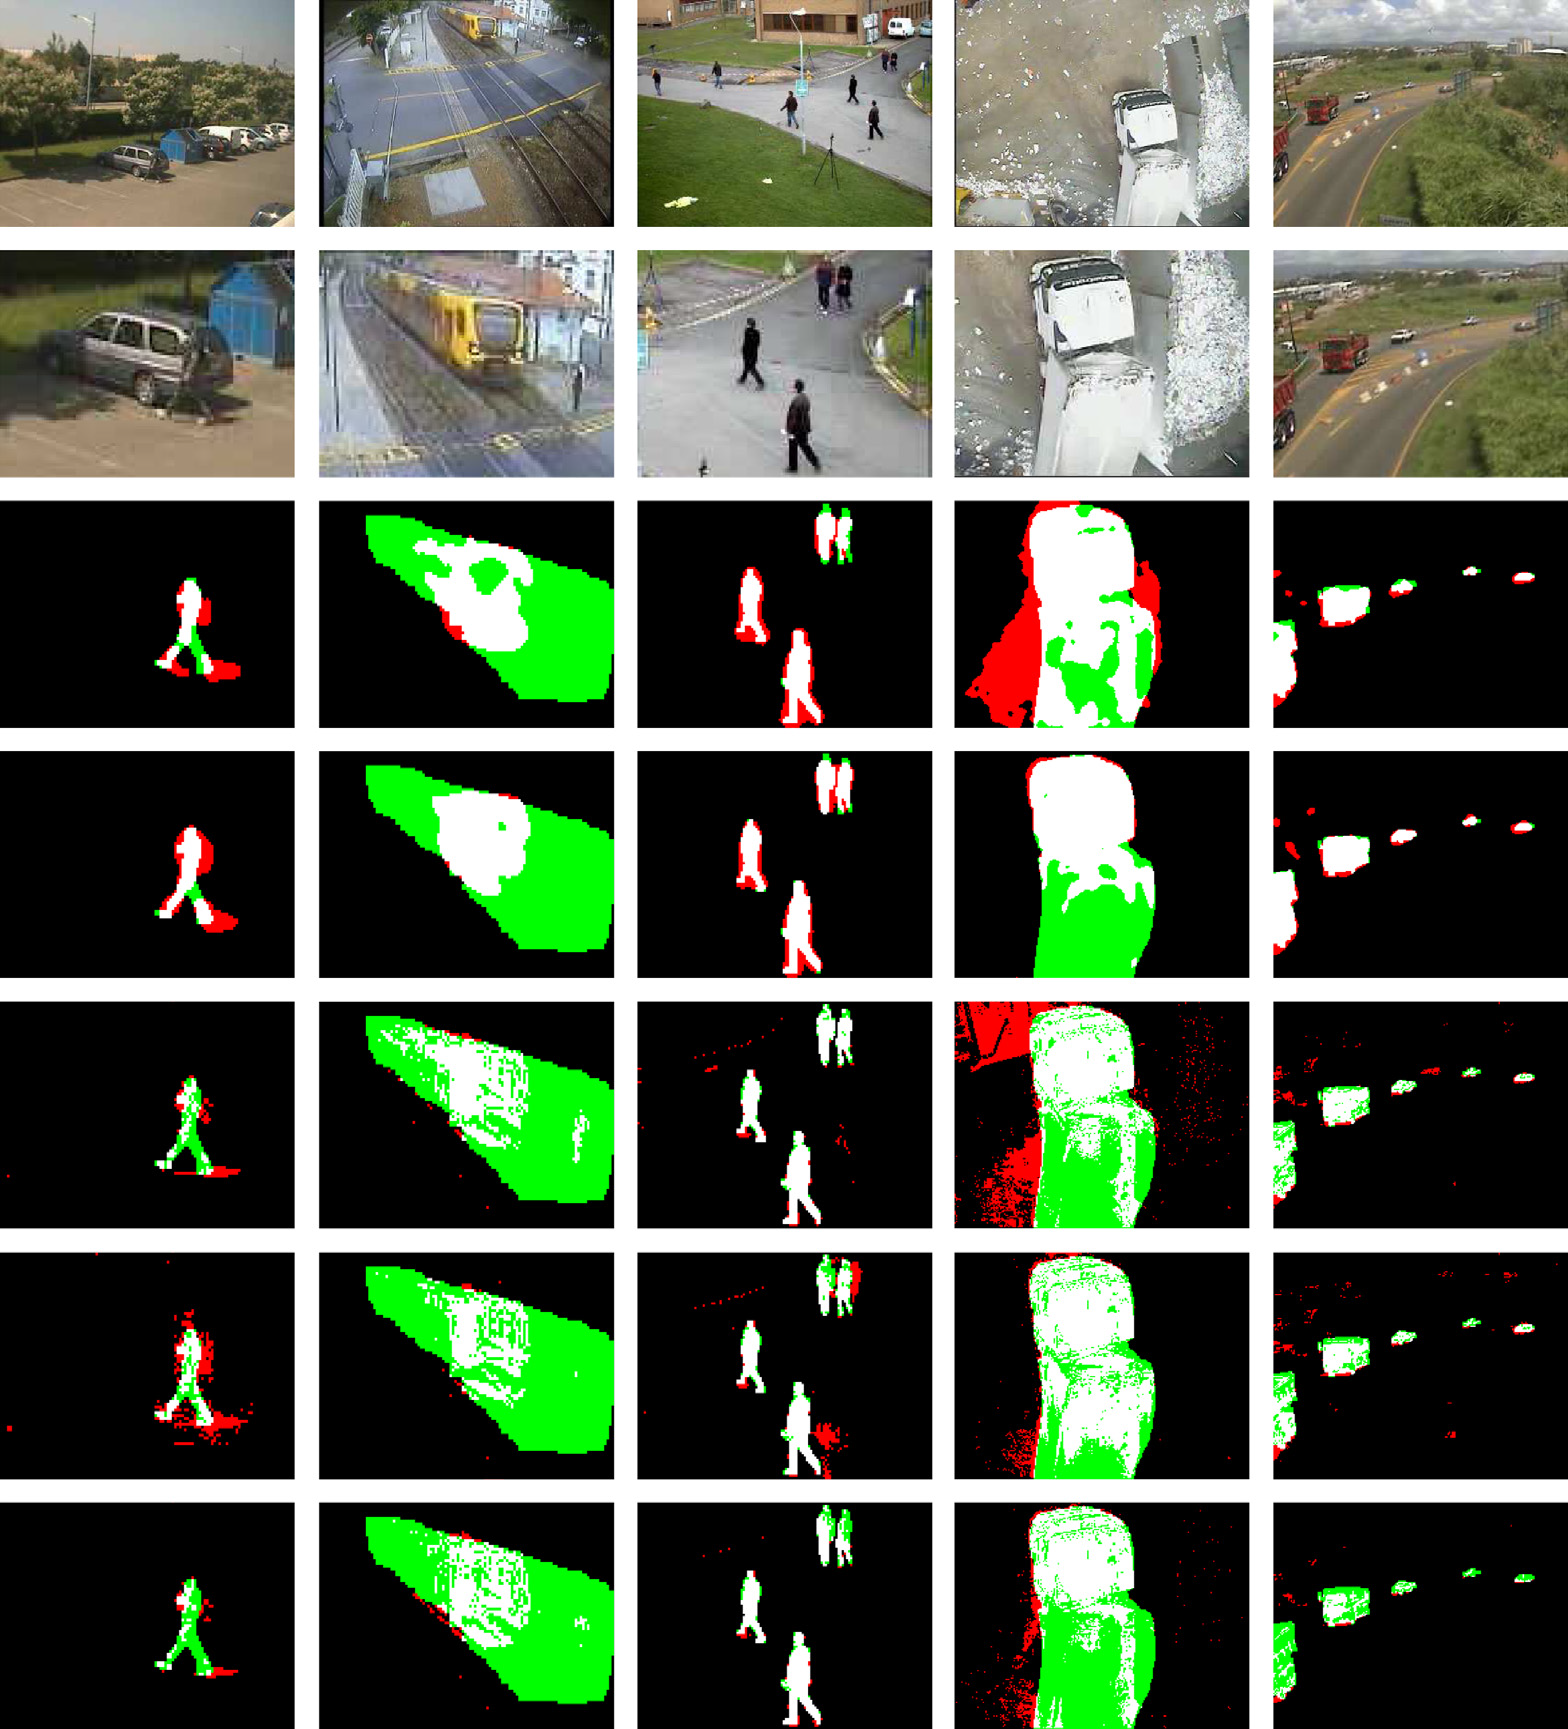
\includegraphics[width=0.9\columnwidth]{bgsreview}
  \caption{Foreground masks obtained from 5 different background subtraction algorithms from real world videos (sourced from \cite{bgs:article}). Images from the first to last row are the input frame, region of interest zoomed in, PBAS, MultiLayerBGS, LBAdaptiveSOM, DPWrenGABGS and MixtureOfGaussianV1BGS algorithms. For the colours, TP pixels are in white, TN pixels are in black, FP pixels are in red, and FN pixels are in green.}
  \label{bgsreview}
\end{figure}

Unfortunately, the PBAS algorithm is no longer available in the BGSLibrary, it is based on the patented ViBE algorithm \cite{barnich2011vibe} therefore was removed \mdc{due to} patent issues. The ViBE algorithm is a powerful background subtraction algorithm with very fast processing speed, high precision and moderate memory usage, the initial implementation is still available, and existed in early versions of OpenCV implemented with CUDA codes runs on GPU.
%}

\iffalse
\subsection{Optical flow}

Optical flow is another widely used object tracking algorithm, it can be used for detect moving objects as well.

There are 2 types of optical flow algorithms. One is sparse feature set (Lucas-Kanade method \cite{bouguet2001pyramidal}), it evaluates pixel movements around selected feature points, therefore calculates movements of feature points. Another type is dense optical flow (Gunner Farneback's algorithm \cite{farneback2003two}), it evaluates pixel movements for all pixels in the frame.

{\color{red}More descriptions and images?}

By rendering pixel movements in 3 axes computed from dense optical flow as 3 components (RGB) colours, then find out regions with the same colour, sizes and positions of moving objects in the scene can then be determined. However, once an object stopped moving, the optical flow algorithms cannot distinguish the object from background any longer.
\fi

\section{Object tracking algorithms}
\label{bg:tracking}

\subsection{Connected component analysis}
\label{blob}

After \mdc{obtaining} the foreground object mask by one of the methods described above, it \modc{needs} to be interpreted as distinct objects, so that the geometry properties of each object can then be retrieved.

Connected component analysis, or connected component labelling, is used for detecting regions that are \moda{different} in some properties, such as colour or brightness. Such a region is also called a blob, which can be the possible presence region of an independent object if applied to the foreground masks. It is very useful to extract parameters such as shape, size and location of the object afterwards.

There are open source blob detection libraries available, such as the simple blob detector came with OpenCV \cite{opencv:blob}, and the cvBlob library \cite{cvblob}. \fref{cvblob} shows an example of tracking blobs by using the cvBlob library.

%{\color{red}Images}

\begin{figure}[H]
  \centering
  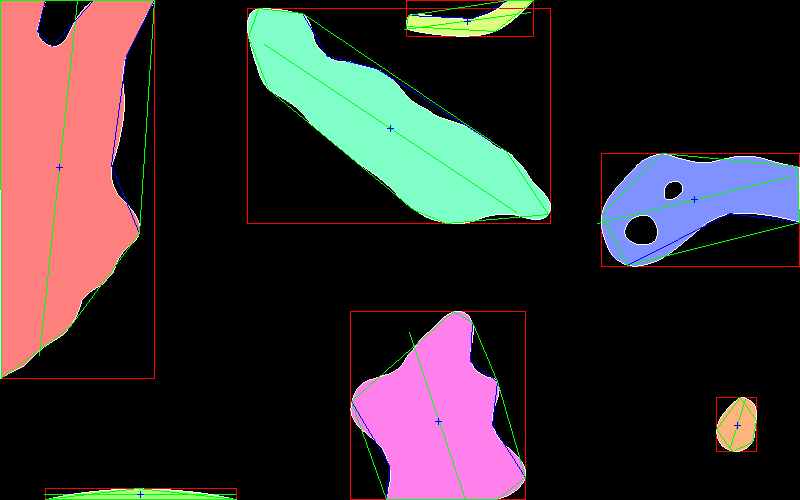
\includegraphics[width=0.7\columnwidth]{cvblob}
  \caption{Tracking blobs with the cvBlob library with bounding shapes, bounding rectangles and blob centres shown (sourced from \cite{cvblob}).}
  \label{cvblob}
\end{figure}

After \modc{determining} the bounding shape, or region of interest (ROI) of an object, the object can then be tracked between adjacent frames by matching the blobs based on similarity in colour and shape or relative position. Movement parameter such as velocity and acceleration may also be obtained by physical modelling.

\subsection{Meanshift and CAMshift}

Meanshift \cite{fukunaga2013introduction} is an algorithm \mdc{which} can be used to track the movement of a fixed size ROI window between adjacent frames. To accomplish this, histogram back projection \mdc{needs} to be applied first to the new frames, which converts the frame to a probability image of each pixels \mdc{belonging} to the target model. Then the meanshift algorithm will be applied to find the peak of probability distribution of the target model. It was implemented within the OpenCV library \cite{opencv:camshift}. \fref{bg:ms:meanshift} shows an example tracking result.

% {\color{red}Images}

Continuously Adaptive Meanshift (CAMshift) \cite{bradski1998computer} is an algorithm based on the Meanshift algorithm, that can handle target object size changing and rotation by iterating over the ROI to find the most suitable configuration. \moda{This algorithm was used by lots of researches for tracking purpose \cite{chu2007object}\cite{xu2012moving}\cite{nouar2006improved}. It was also implemented in the OpenCV library \cite{opencv:camshift}.}. \fref{bg:ms:camshift} shows an example tracking result, \mdc{compared} to the Meanshift algorithm tracking (\fref{bg:ms:meanshift}), it can resize and rotate ROI automatically.

\begin{figure}[H]
  \centering
  \subfigure [] {
    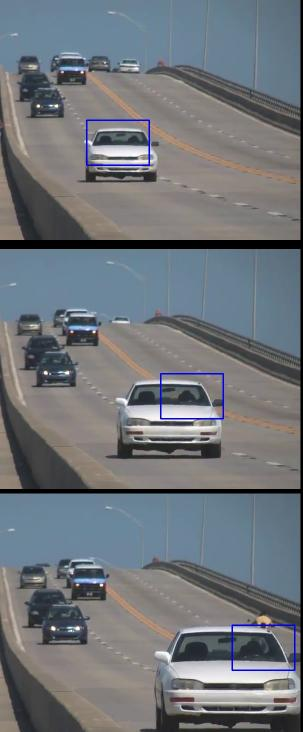
\includegraphics[width=0.3\columnwidth]{meanshift_result}
    \label{bg:ms:meanshift}
  }
  \subfigure [] {
    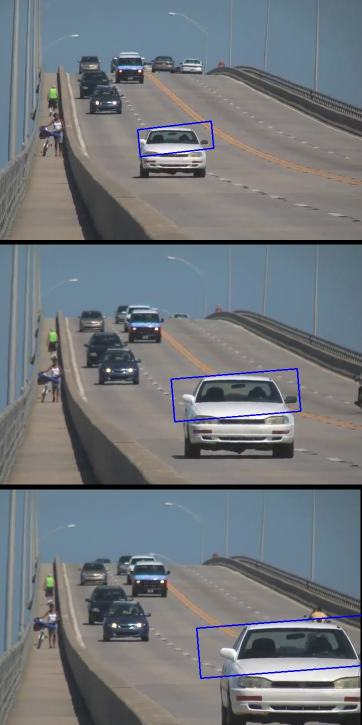
\includegraphics[width=0.35\columnwidth]{camshift_result}
    \label{bg:ms:camshift}
  }
  \caption{Meanshift and CAMshift tracking examples (sourced from \cite{opencv:camshift}). \subref{bg:ms:meanshift} shows the Meanshift tracking, \subref{bg:ms:camshift} shows the CAMshift tracking.}
  \label{bg:ms}
\end{figure}

%{\color{red}Images}

\subsection {Optical flow}

%By evaluating pixel movements of feature points inside ROI, the speeds of moving objects projected onto camera sensor can be determined.

Optical flow is another widely used object tracking algorithm that evaluates pixel moving around feature points, by assuming neighbouring pixels will have similar motion as the feature points. Although it can also be used for detecting moving objects by considering regions of points with the same motion as one moving object, once the object stopped moving, the optical flow algorithms cannot distinguish the object from background any longer. Therefore it is mainly used for object tracking rather than detection.

There are 2 types of optical flow algorithms. One is sparse feature set (Lucas-Kanade method \cite{bouguet2001pyramidal}), it estimates pixel movements around selected feature points. To determine feature points, OpenCV implemented a good features to track \cite{shi1994good} algorithm to find the strongest corners in an image. After that, by moving the feature points according to the movements computed, the object can be tracked across sequence of video frames, as shown \mdc{in} \fref{bg:of:opticalflow_lk}.

Another type is dense optical flow (Gunner Farneback's algorithm \cite{farneback2003two}), it evaluates pixel movements for all points in the frame. \fref{bg:of:opticalfb} shows the result from a dense optical flow tracking scene by rendering movements in 3 axes as red, green and blue components respectively.

\begin{figure}[H]
  \centering
  \subfigure [] {
    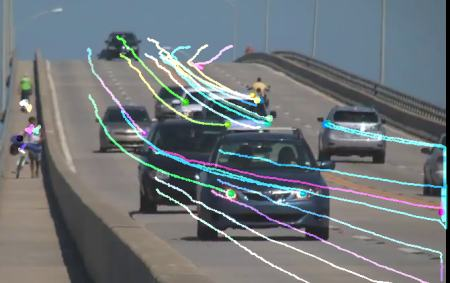
\includegraphics[width=0.3\columnwidth]{opticalflow_lk}
    \label{bg:of:opticalflow_lk}
  }
  \subfigure [] {
    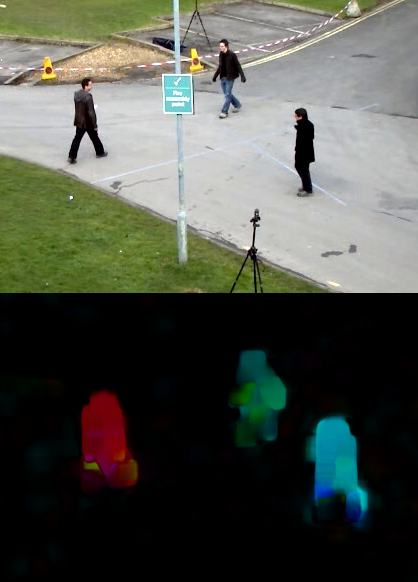
\includegraphics[width=0.3\columnwidth]{opticalfb}
    \label{bg:of:opticalfb}
  }
  \caption{Optical flow example scenes (sourced from \cite{opencv:of}). \subref{bg:of:opticalflow_lk} shows the sparse feature set (Lucas-Kanade method), \subref{bg:of:opticalfb} shows the dense optical flow (Gunner Farneback's algorithm).}
  \label{bg:of}
\end{figure}

% {\color{red}More descriptions and images?}

% {\color{red}Images}

\section{Object recognition}

Object recognition can also be developed by applying different cascade classifiers as described previously in section \ref{sec:bg:cc} to the ROI of the specific object. This process is very computation intensive and time consuming, therefore should be executed as few as possible to \modc{save energy consumption}. \moda{For example, only execute object recognition once the object first enters the sense, or execute to the frame with the maximum visible size of the target object.}

\section{Automatic feedback control}

\mdc{There are researches} about energy-efficient object detection by utilising hardware-level operations \cite{casares2011energy}. \modc{This research \cite{casares2011energy}} had achieved energy consumption reduction by $54.136\%$. However, it was done on a very different and limited platform, based on a very limited algorithm, possible to extend to algorithms with more general usage.

\section{Sample video datasets}

There are sample video datasets proposed for testing, evaluating and comparing computer vision algorithms, specifically background subtraction algorithms. The resolutions are $320 \times 240$ typically, up to about $720 \times 480$, with frame rates of $30$ frames per second (FPS) mostly.

For example, ChangeDetection.NET(CDNET) \cite{goyette2012changedetection} and Background Models Challenge \cite{vacavant2012benchmark} provides realistic camera-captured videos with lots of diverse sets of scenarios and high quality ground truth masks, while Stuttgart Artificial Background Subtraction Dataset \cite{brutzer2011evaluation} was using 3D models and ray tracing technology to generate artificial but realistic videos of typical video surveillance scenarios.

\chapter{Design} \label{Chapter:Design}

\section{Specification}

% {\color{red}Specification of works, quantifiable}

\begin{itemize}
	\item Customise a NVIDIA Jetson TK1 embedded board and its Linux operating system for power efficiency.
	\item Interface an OV5647 camera to the target platform through MIPI-CSI interface and V4L2 driver platform.
	\item Configure the camera including different resolution modes through V4L2 interface.
	\item Capture still images and video sequences with the camera through V4L2 interface.
	\item Control the camera frame rate while the camera is actively capturing video stream.
	\item Implement object tracking algorithm on the target platform for video surveillance application.
	\item Optimise the algorithm so that it runs around $30$ FPS on the platform.
	\item Achieve $50\%$ power saving on some typical real world video surveillance dataset through adaptive operation.
	\item Maintaining $80\%$ successful object tracking rate with the adaptive operation.
	\item Build a camera and algorithm power consumption model.
	\item Use the model to estimate power saving achieved through adaptive operation.
\end{itemize}

\section{Hardware}

% {\color{red}Design works, choices of hardware, software, etc.}

\subsection{Hardware platform}

%ARM or x86?

An embedded development board was used in this project, it enables easy power consumption analysis and is more likely the situation where power efficiency will be required rather than a desktop or server environment.

The most broadly used and powerful embedded processor architecture is ARM. It has relatively high performance grade available, extensively hardware and software support including embedded Linux operating system with reasonable power consumption and varies power saving modes, therefore was chosen to be used in this project.

Specifically, the Jetson Tegra K1 embedded development platform \cite{NVIDIA:tk1} featuring a 2.32GHz quad-core ARM CPU and a CUDA enabled Tegra GPU, introduced by NVIDIA, was used in this project. It has a rich set of peripheral interfaces exported enables low-level control and interfacing with a MIPI-CSI high resolution camera module and is powerful enough to develop programs and execute complex computer vision algorithms on board. The heterogeneous architecture with CUDA enabled GPU can also be fully utilised by the GPU module in the specifically optimised OpenCV library, makes it particularly suitable for computer vision tasks.

There are other heterogeneous architecture embedded platforms with ARM CPU cores and ARM GPUs available, but ARM GPUs are currently not supported by OpenCV's GPU module, and the CPUs alone are probably not powerful enough for complex computer vision tasks.

% {\color{red}More}

A general x86 architecture computer running Microsoft Windows operation system with a webcam was also used for algorithm development and remote control of the embedded development board. Since most algorithm developments do not use platform specific features, they can be developed on a general computer then easily migrated to the embedded platform.

\subsection{Camera}

% Specific camera module to be used was not determined yet at the time this progress report was written, but it would be a high resolution camera module from OmniVision \cite{ovt} that can be easily interfaced and directly controlled with the peripheral interfaces on the Jetson TK1 platform. A Linux kernel module driver probably need to be developed in order to control the camera parameters and operations from program running in user space.

The raspberry pi camera module was used in this project, it features a 5 mega pixels OV5647 camera sensor manufactured by OmniVision Technologies Inc. It is relatively more expensive than buying the camera sensor only, but the raspberry pi camera module is more broadly available in small quantities and can be easily connected to the board without the need to design a dedicated adapter PCB. It uses the MIPI-CSI interface which the board has native support for, the complete data sheet is also available around the Internet and it features subsampling, frame rate control, auto exposure and white balance functions etc. which are essential to adaptive operation.

The only difficulty is that the camera sensor can only output frames in raw Bayer pattern format \cite{bayer1976color}, but since the format can be efficiently converted using the GPU cores and CUDA, that is not a significant issue.

\section{Software}

\subsection{Operating system}

Ubuntu Linux distribution version 14.04.1 LTS was used on the platform, installed directly from the file system image provided by NVIDIA. Linux is great for this project because it is fully configurable, so that operating system overheads can be reduced to minimum by disabling unused services, even the graphical desktop environment. Also most Linux operations can be done through just command line interface, possibly via a SSH shell access, therefore programming and controlling the platform can be done anywhere with internet connection, which is very convenient.

The open-source GNU/Linux system also provides familiar and widely used tool sets, kernel driver development is well-documented, cross platform computer vision libraries especially OpenCV is also available, and has enormous community support.

\subsection{Computer vision API}

OpenCV \cite{opencv} was used to implement the algorithms, due to its cross platform adaptability, easy to use and has large number of efficient algorithms ready for use and analysis. Furthermore, the OpenCV library for Jetson platform provided by NVIDIA had been further optimised, provides 2x-5x speed up compare to regular OpenCV \cite{NVIDIA:perf}. The OpenCV GPU module based on NVIDIA CUDA was also available, utilises the heterogeneous architecture and provides 5x-20x speed up. These optimisations can reduce computation time dramatically, thus further reduces the power consumption.

\subsection{Testing dataset}

Using a consistent video stream input and a camera power consumption model instead of replaying the same scene in front of the camera is preferred, because reproducing the exactly same video stream from replaying scene is impossible, factors such as camera and object instability, inaccurate synchronisation, hardware and software restrains will also take effect.

The video database from \cite{goyette2012changedetection} was used for testing the algorithms and analysing the performance and accuracy of adaptive operation. The database was rigorous and comprehensive, involves lots of carefully chosen video streams from different real life scenarios, very useful for evaluate object tracking algorithms in different situation.

\section{Algorithms}

\subsection{Object detection algorithm}

The model based object detection algorithms described in previous chapter might be useful for some specific projects, but for a more general object tracking system with previously specified application areas, motion based algorithms which can track any kind of moving objects, was used in this project for evaluating adaptive operation.

There are 2 possible motion based object detection algorithms described previously, background subtraction and optical flow. Since optical flow can only detect moving objects, objects moving in a relatively low speed or stops for a few moments, which are common in a lot of scenarios would be undetectable by optical flow, therefore background subtraction that can handle this kind of situations was used for the object detection phase.

However, there are several distinctive background subtraction algorithms available for use. After some evaluations, the ViBE algorithm was chosen, because it is relatively efficient, with moderate memory usage and has GPU implementation, thus can take the advantage of heterogeneous platform architecture.

\subsection{Object tracking algorithm}

Connected component analysis is used after foreground masks being extracted from each frame. Specifically, the simple find contour function that is also used by the simple blob detector from OpenCV was used. It is very simple, but still sufficient to extract blobs from black and white masks without intensive computation.

Afterwards, the good features to track function is used to determine feature points inside foreground masks, then related to the objects detected respectively. After that, sparse set optical flow will be applied to track the movements of feature points in following frames. By relating the feature points back to objects, the objects can then be tracked.

% {\color{red}HOW???}

\chapter{Implementation}

\section{Camera module}

\modc{\subsection{Hardware connection}}

The Raspberry Pi camera module was connected to the Jetson TK1 board as shown \mdc{in} \fref{imp:schematic}\modc{, \fref{imp:connection}}. A 74HCT245 bus transceiver chip was used as a buffer for voltage level conversion, since GPIOs on the Jetson board are using $1.8V$ voltage level while the Raspberry Pi module is working at $3.3V$ voltage level. \modc{The camera needs 2 discrete interfaces for control and communicate, I2C and MIPI-CSI. I2C interface is a relatively low speed interface with multi master and multi slave addressing support, is used to control and configure the camera. MIPI-CSI interface is a high speed data transmission interface designed for high resolution cameras, by having multiple differential data lanes to multiple maximum transmission speed. The camera uses 2 data lanes to transmit frame data and synchronise.}

\begin{figure}[htb]
  \centering
  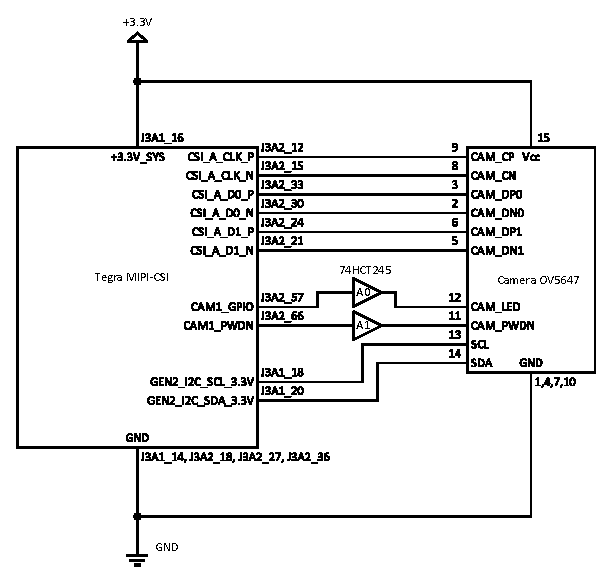
\includegraphics[width=0.7\columnwidth]{schematic}
  \caption{Schematic of Jetson board connect to a Raspberry Pi camera module.}
  \label{imp:schematic}
\end{figure}

\modc{\begin{figure}[htb]
  \centering
  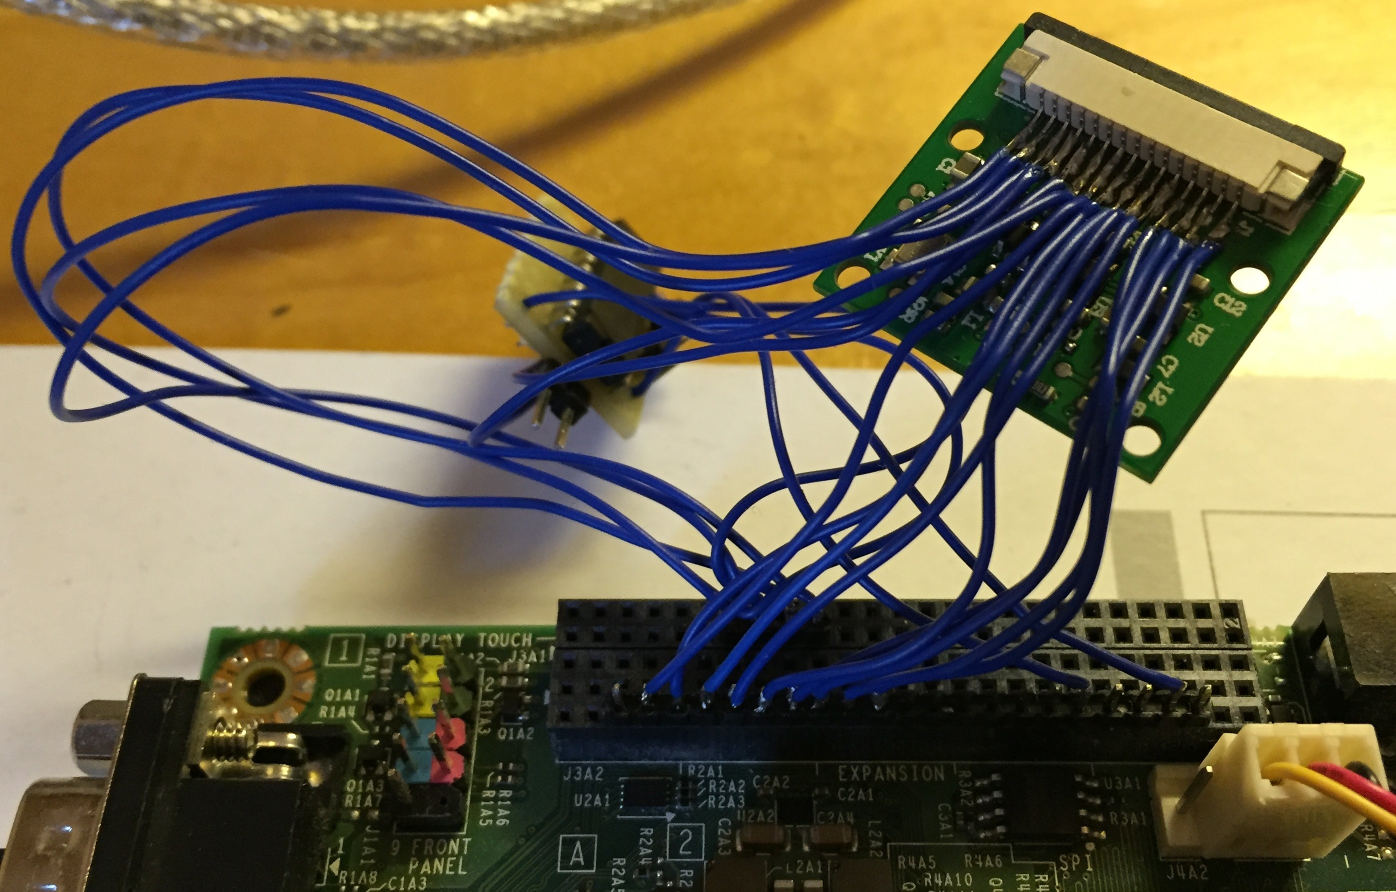
\includegraphics[width=0.7\columnwidth]{connection}
  \caption{Photo of the connection between the camera model and the Jetson board.}
  \label{imp:connection}
\end{figure}

The camera module is using an on-board $25 MHz$ oscillator, then multiplied to $48 MHz$ pixel clock by Phase Locked Loop (PLL) inside the camera sensor. Changing of frame interval was done by adding dummy blank lines after frame data.

The GPIO on the camera module is controlling \mdc{an} LED mounted on the module, and it is controllable through the camera driver. Therefore by controlling the GPIO, it not only \mdc{can give} indications about camera activity, but also is very useful for debugging and triggering external power analyser.

%{\color{red}Camera waveform.}

\fref{imp:cam:osc} shows a detailed waveform captured using an oscilloscope during camera frame rate configuration. The camera resolution was configured to a higher resolution mode for 2 frames, then changed back. Frame data, line data, synchronisation packet and I2C transmissions are clearly marked on the waveform.

\begin{figure}[htb]
  \centering
  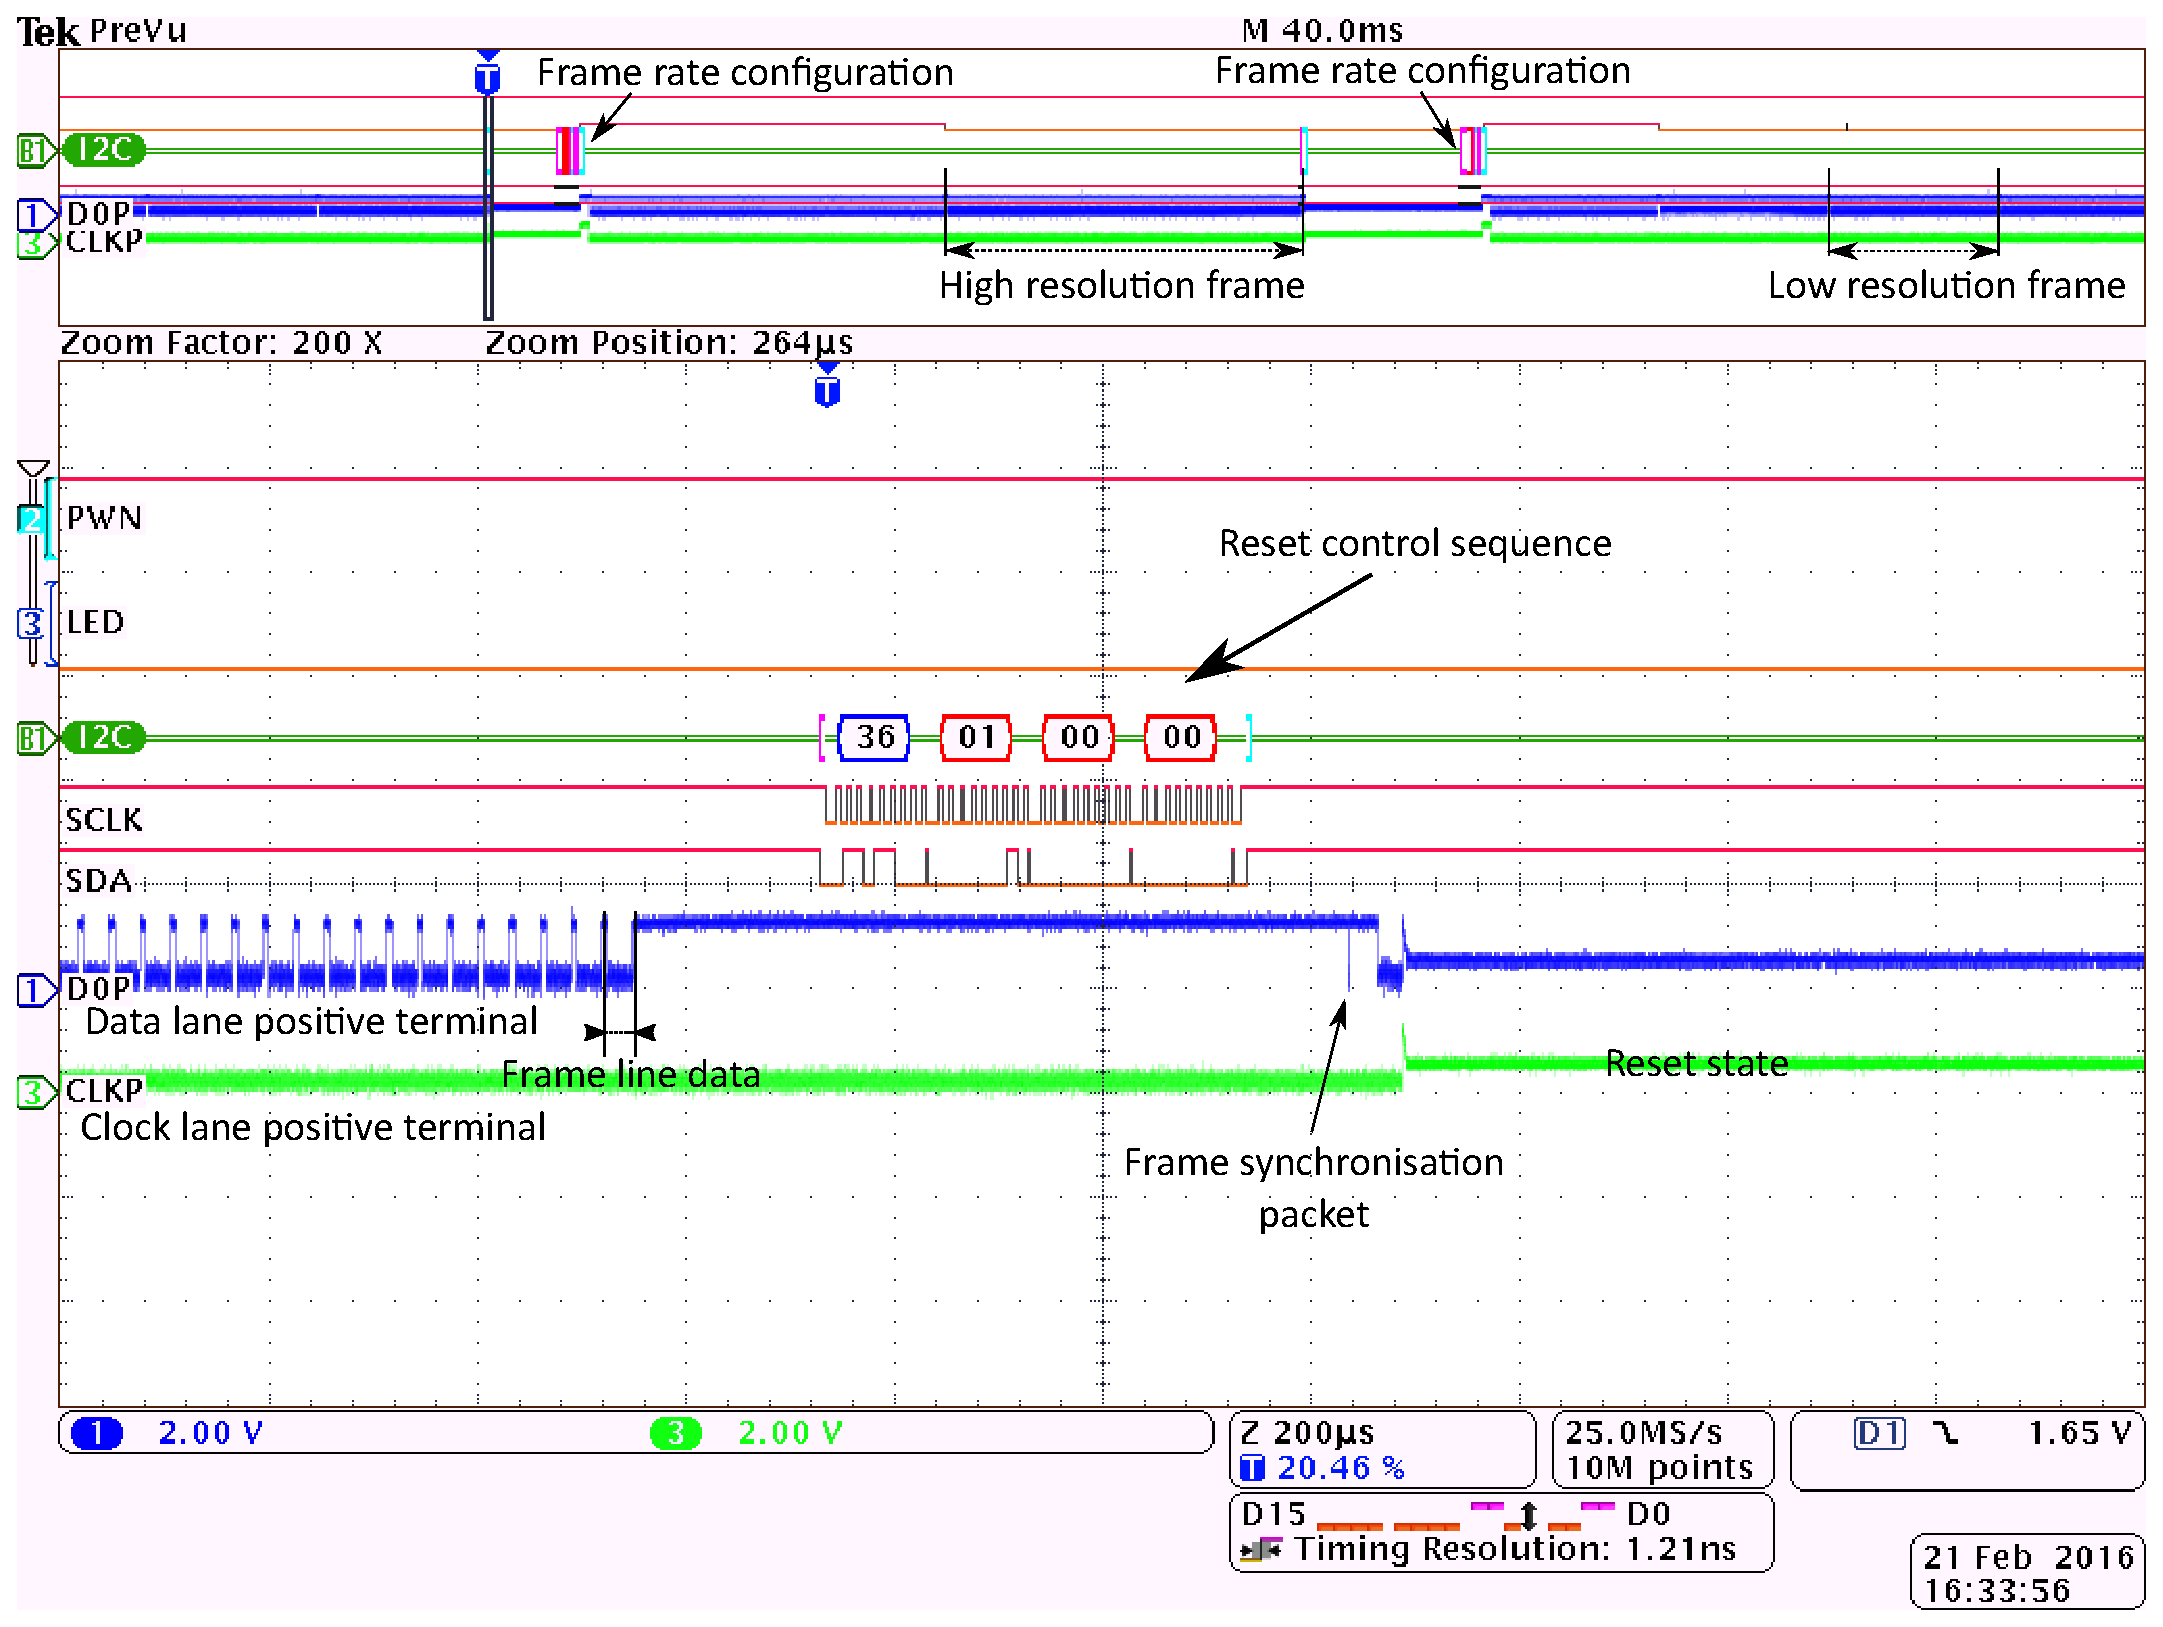
\includegraphics[width=\columnwidth]{cam_osc}
  \caption{Waveform capture of configuring camera module.}
  \label{imp:cam:osc}
\end{figure}

\subsection{Driver development}}

The camera driver was implemented based on Linux Video for Linux second version (V4L2) framework. It is a great framework that supports \mdc{various} kinds of different camera sensor models with the same user space interface, across vast number of different embedded Linux platforms, \mdc{enabling} cross platform adaptability with accessibility to low level controls.

The V4L2 interface driver on the Jetson platform is composed by 3 different drivers, as shown \mdc{in} \fref{imp:drivers}. Upon system \moda{start-up, \mdc{various} external hardware modules' electrical connection information, that are stored in a board specific initialisation file, will be loaded as platform drivers. For the camera module, I2C peripheral address and MIPI-CSI data lane usage information are required.} Later when soc\_camera driver loads, it will use those informations to try to active corresponding sub-device control drivers, the connection configurations will also be passed to the control drivers. The control drivers can only \mdc{control} I2C interfaces to access camera registers, while MIPI data lanes and capture buffers are managed by another independent driver.

\begin{figure}[H]
  \centering
  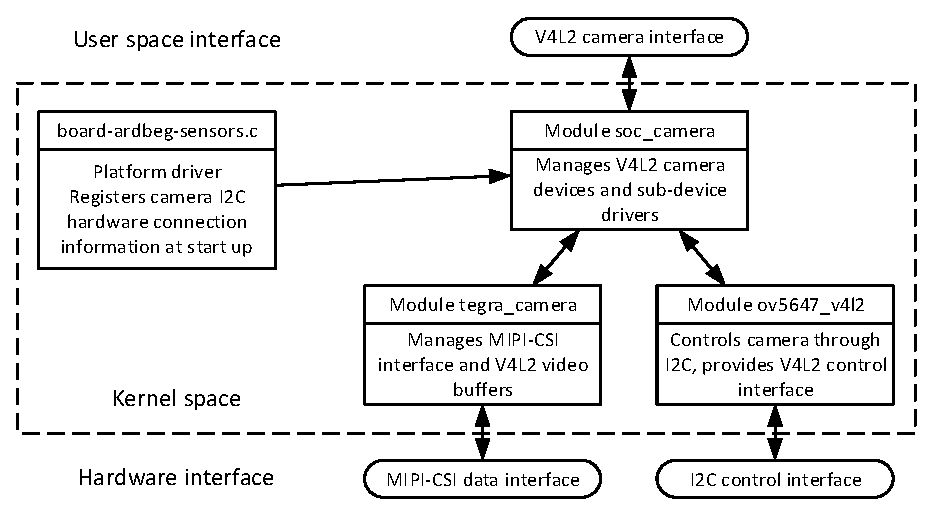
\includegraphics[width=0.7\columnwidth]{drivers}
  \caption{Structure of V4L2 interface drivers on Jetson board.}
  \label{imp:drivers}
\end{figure}

The soc\_camera top module and capture buffer management module are already provided by NVIDIA, therefore only the platform driver and control driver \moda{are} required to be implemented.

For adaptive operation, the driver implemented supports different resolution modes available from the camera and precise frame interval alteration. A special control instruction that can change any of the control registers inside the camera sensor was also developed for debugging and controlling \mdc{purposes}.

\section{Application}

% {\color{red}Application structure, multithreading}
% Bayer pattern handling.
% Multi-threading:
% 	i. Camera thread for camera control, buffer swapping, synchronisation and management etc.
% 	ii. OpenGL preview thread shows the camera output in real time, can be suspended for power saving.
% 	iii. OpenCV worker thread running algorithms.
% 	iv. OpenCV viewing thread.
% 	Display results and handle GUI user input, slow, can be suspended for power saving.

\subsection{Bayer pattern handling}

Initially, for capturing still images and OpenGL video preview, the conversion from Bayer pattern to RGB colour space was implemented. Later in OpenCV processing, it was accomplished through OpenCV's built-in functions directly.

To convert a Bayer pattern image to RGB space, a $3 \times 3$ square of pixels around the target pixel is needed. By averaging surrounding pixels according to \fref{imp:bayer4}, RGB values of each pixel can be approximated.

\begin{figure}[H]
  \centering
  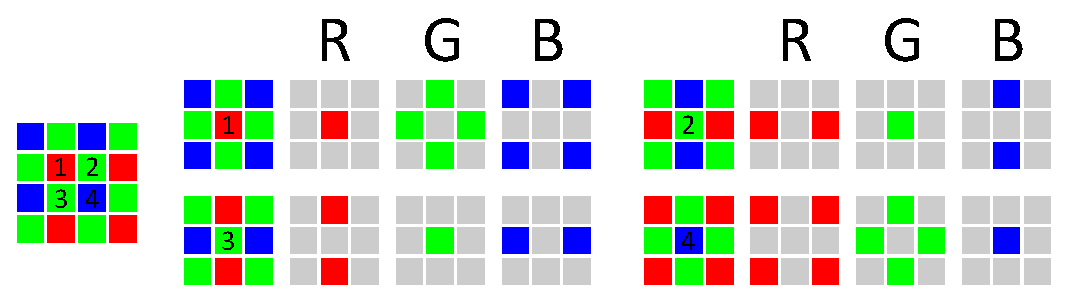
\includegraphics[width=\columnwidth]{bayer4}
  \caption{4 different situations in Bayer pattern to RGB colour space conversion.}
  \label{imp:bayer4}
\end{figure}

\fref{imp:bayer_eg} shows a detailed fraction of a test pattern generated by the camera sensor, and Bayer to RGB colour space conversion result.

\begin{figure}[H]
  \centering
  \subfigure [] {
    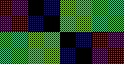
\includegraphics[width=0.4\columnwidth]{bayer_raw}
    \label{imp:bayer_raw}
  }
  \subfigure [] {
    
\includegraphics[width=0.4\columnwidth]{bayer_res}
    \label{imp:bayer_res}
  }
  \caption{Test pattern generated by the camera sensor. \subref{imp:bayer_raw} the generated Bayer pattern, \subref{imp:bayer_res} RGB colour space conversion result.}
  \label{imp:bayer_eg}
\end{figure}

% A typical colourful computer image consists of 3 primary colour channels {\color{red}CITE}, which are red, green and blue. However, because of physical and manufacture constrains, most of camera sensors including the camera used in this project have only one intensity sensor per pixel of a specific colour, arranged in a special pattern called Bayer pattern {\color{red}CITE}, therefore image processing algorithm need to be applied to convert or approximate the raw data to produce full colour images. Some of the camera sensors have a built-in image processor that applies the algorithm automatically, but the camera used in this project doesn't have that functionality, therefore the algorithm need to be implemented by the application.

%{\color{red}Some diagrams show how it is done.}

\subsection{Application structure}

An application was developed to receive video stream from \moda{a camera module} or from a testing dataset, then apply OpenCV processing, real-time input and output video preview as well as adaptive camera control. To take the benefits of the heterogeneous architecture more efficiently and overcome issues with buffer updates, the application was implemented using multi-threading approach with inter-thread synchronisation mechanisms.

The main thread in camera mode is responsible for initialisation, camera control, capture buffer synchronisation and management. It allocates several buffers for the camera driver, \mdc{assigns} filled buffers to other processing threads and \mdc{recycles} processed buffers back to camera driver. In dataset mode it reads the sequence of frames, skips frames according to frame rate set by adaptive operation. \modc{The timestamps of video buffers were also recorded, so that exact time between 2 frames can be calculated for adaptive operation.}

After \mdc{obtaining} a frame from video stream, an OpenGL live video preview thread was then used to show the frame to a monitor, independent from the processing algorithm. This thread can be independently stalled so that it would not consume any processing power when analysing performances and power consumptions of algorithms. In camera mode, it will convert the frames received from Bayer pattern format to RGB colour space for rendering onto the screen. This process is done by GPU through OpenGL shaders, therefore is extremely fast, around 200 FPS for $640 \times 480$ resolution if synchronisation with main thread is disabled.

The OpenCV algorithms \mdc{run} on both CPU and GPU, and OpenCV has a \mdc{constraint} that \mdc{is} to view the processed images, the application needs to call a user interface update function that is time consuming but not power intensive, therefore 2 threads \mdc{were} used in a pipeline style in order to speed up the processing. The buffers received from main thread will first go through the processing thread, then pass to the second thread for display on the monitor. The display thread can also be stalled for power saving.

%The OpenCV algorithms runs on both CPU and GPU, therefore to take the full advantages of heterogeneous architecture and run the algorithms as fast as possible, the OpenCV processing runs in a pipelined style through 3 threads. Every buffer received will go through first CPU processing thread, then transferred to GPU processing thread, finally .
%and OpenCV has a constraint that to view the processed image results, the application, so that two OpenCV processing threads was created so that.

Finally, \mdc{there is} an input \mdc{handling} thread for debugging and controlling through command line interface. Most of \mdc{the} time this thread \modc{waits} for user input, therefore won't consume considerable CPU time.

\section{Object detection algorithms}

\subsection{Colour based}

A simple implementation of colour filtering object detection algorithm \cite{MOTBOC.git} was investigated, as shown in \fref{imp:MOTBOC}.

However, this implementation is very limited, it can only \mdc{detect} objects with single colour, \modc{and it} cannot distinguish the objects from similar background colour, relies heavily on manually adjusted colour threshold values, very sensitive to the variations of colour from different cameras and environment lighting conditions, therefore not very adaptable. A complex environment may also \mdc{result in} undesired detections, as shown in \fref{imp:MOTBOC_F}. Background objects that \mdc{have a} similar colour to the desired red objects were detected as foreground red objects, and some target objects were not been identified and misclassified because of \mdc{a} slight change in \mdc{the} lighting condition, the objects' colour seen by the camera \mdc{was} no longer inside the colour filters' ranges.

\begin{figure}[H]
  \centering
  \subfigure [] {
    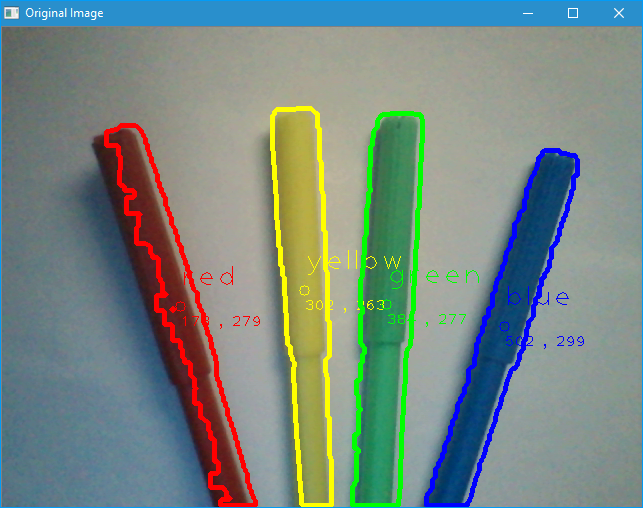
\includegraphics[width=0.4\columnwidth]{MOTBOC_imp}
    \label{imp:MOTBOC_}
  }
  \subfigure [] {
    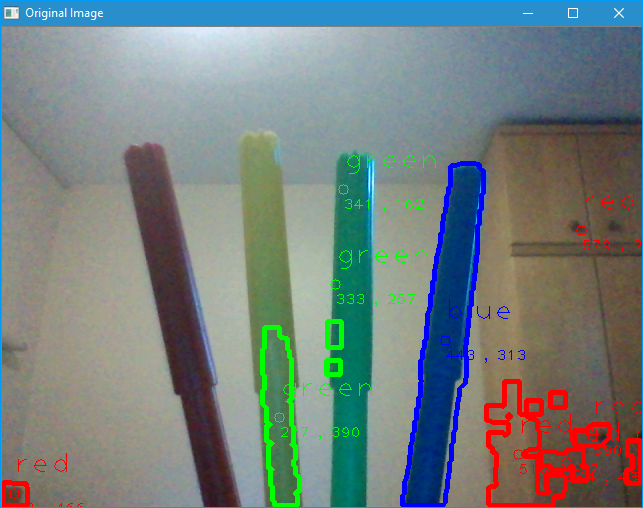
\includegraphics[width=0.4\columnwidth]{MOTBOC_fail}
    \label{imp:MOTBOC_F}
  }
  \caption{Simple multi object tracking based on colour \cite{MOTBOC.git}. \subref{imp:MOTBOC_} ideal situation, \subref{imp:MOTBOC_F} messed up in a complex environment with slightly different lighting condition.}
  \label{imp:MOTBOC}
\end{figure}

\subsection{Circle detection}

OpenCV's implementation of Hough Circle Transform for circle detection was investigated, as shown \mdc{in} \fref{Figure:circles}.

%\fref{Figure:circles} shows the image processed by circle detection, based on OpenCV's implementation of Hough Circle Transform \cite{opencv:hough_circle}.

\begin{figure}[H]
  \centering
  \subfigure [] {
    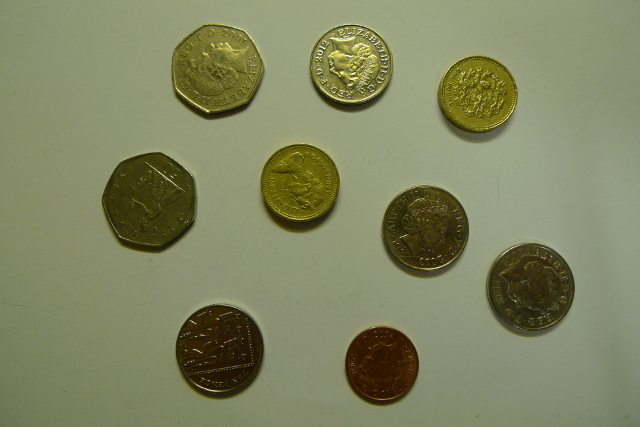
\includegraphics[width=0.45\columnwidth]{simple_original}
    \label{Figure:edges:original}
  }
  \subfigure [] {
    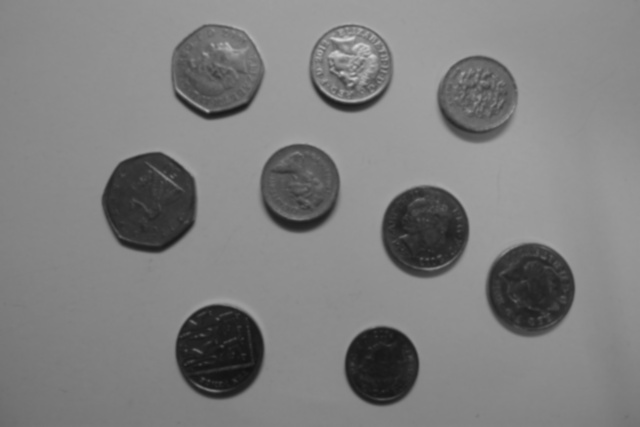
\includegraphics[width=0.45\columnwidth]{simple_blur}
    \label{Figure:edges:blur}
  }
  \subfigure [] {
    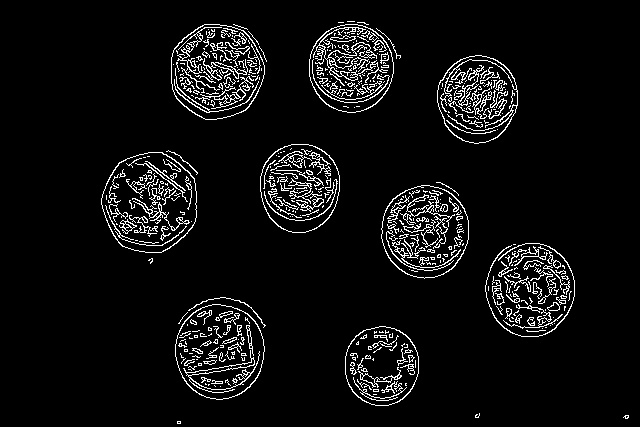
\includegraphics[width=0.45\columnwidth]{simple_edges}
    \label{Figure:edges:edges}
  }
  \subfigure [] {
    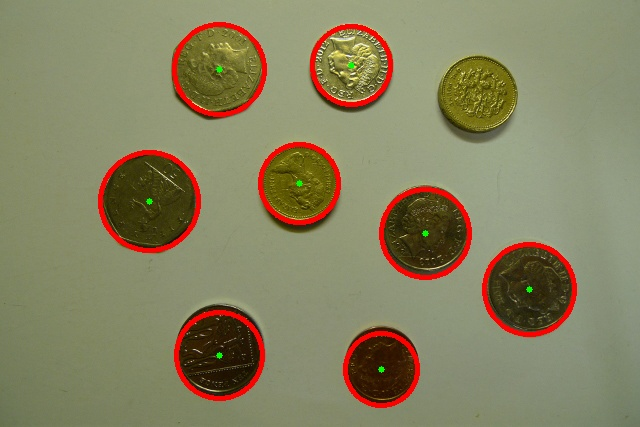
\includegraphics[width=0.45\columnwidth]{simple_circles}
    \label{Figure:edges:circles}
  }
  \caption{Circle detection. \subref{Figure:edges:original} The original image, \subref{Figure:edges:blur} image converted to gray scale and blurred, \subref{Figure:edges:edges} edges extracted, \subref{Figure:edges:circles} circles detected}
  \label{Figure:circles}
\end{figure}

The frame captured from camera (\fref{Figure:edges:original}), was first converted to grey scale then blurred, as shown in \fref{Figure:edges:blur}. Blur or smoothing is necessarily to reduce false object edges that might be detected. Afterwards the object edges in the image \mdc{were} extracted as in \fref{Figure:edges:edges}. Finally \fref{Figure:edges:circles} shows the circles detected by the algorithm.

However, this algorithm is still very limited and inaccurate, as shown \mdc{in} \fref{Figure:circles}, the coin at the top right corner had not been detected, because it appeared to be an ellipse instead of a prefect circle because of \mdc{the} camera perspective. Furthermore, in order to detect multiple geometric shapes, different algorithms would be required for each of the different shapes.

\subsection{Cascade Classifier}

% as shown in \fref{Figure:cc_face}

The OpenCV's cascade classifier implementation \cite{opencv:cc} of face and eye detection \mdc{were} investigated as shown in \fref{Figure:cc_face}.

\begin{figure}[H]
  \centering
  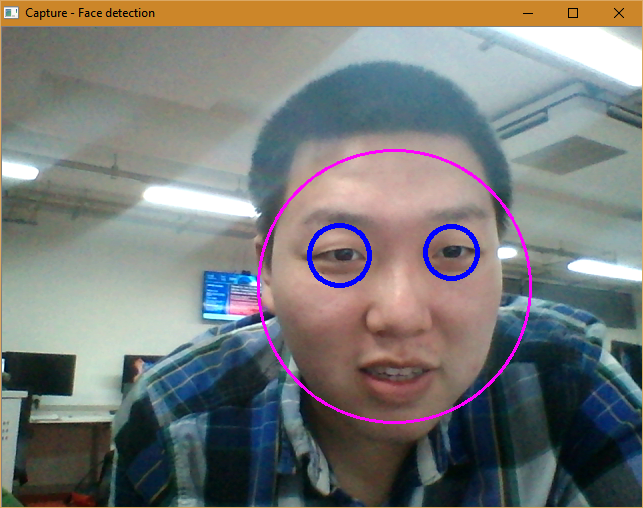
\includegraphics[width=0.6\columnwidth]{cc_imp_face}
  \caption{Face and eye detection cascade classifiers, detected face was circled by pink, whereas detected eyes were circled by blue}
  \label{Figure:cc_face}
\end{figure}

Noticeable frame rate drop \modc{(only about 3 fps) was} experienced when running the cascade classifier implementation on the testing platform, \mdc{suggesting that} it might not be a suitable algorithm for real-time object tracking application on embedded platforms.

\moda{\subsection{Motion based background subtraction}}

4 out of the 5 best algorithms reviewed by the article \cite{bgs:article} that are available in the BGSLibrary as listed in \tref{Table:bgs} were investigated in this project.

%{\color{red}GPU implementation?}

%\iffalse
\begin{table}[H]
  \centering
  \begin{tabular}{cc}
  \toprule
  \textbf{Method ID} & \textbf{Method name}\\
  \midrule
  MultiLayerBGS & Multi-Layer BGS \\
  MixtureOfGaussianV1BGS & Gaussian Mixture Model \\
  LBAdaptiveSOM & Adaptive SOM \\
  DPWrenGABGS & Gaussian Average \\
  \bottomrule
  \end{tabular}
  \caption{Background substraction algorithms investigated (adapted from \cite{bgslibrary})}
  \label{Table:bgs}
\end{table}
%\fi

%The missing Pixel-Based Adaptive Segmenter (PBAS) algorithm , because the algorithm is based on patented ViBE algorithm, therefore removed from the BGSLibrary to avoid patent issue. However,

The ViBE algorithm from early versions of OpenCV as a non-free add-on module implemented with CUDA runs on GPU, which is also the base of the missing PBAS algotihm, was also investigated.

\fref{Figure:bgs_frame} shows the foreground masks obtained at the same frame index by those 5 algorithms. The dataset used are 2 sample highway surveillance video datasets came with the BGSLibrary \cite{bgslibrary}.

\begin{figure}[htb]
  \centering
  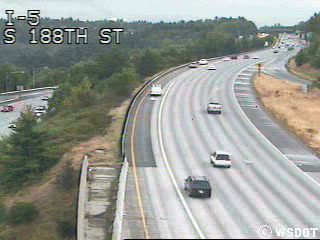
\includegraphics[width=0.3\columnwidth]{bgs_frame/input}
  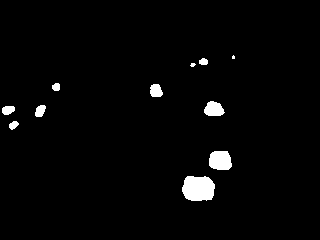
\includegraphics[width=0.3\columnwidth]{bgs_frame/MultiLayerBGS/mask}
  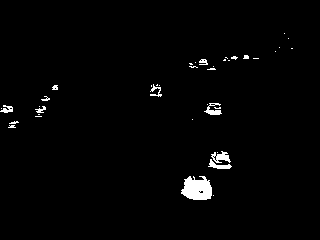
\includegraphics[width=0.3\columnwidth]{bgs_frame/MixtureOfGaussianV1BGS/mask}
  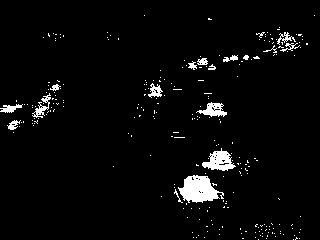
\includegraphics[width=0.3\columnwidth]{bgs_frame/LBAdaptiveSOM/mask}
  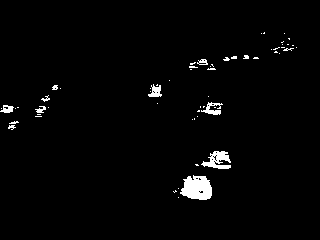
\includegraphics[width=0.3\columnwidth]{bgs_frame/DPWrenGABGS/mask}
  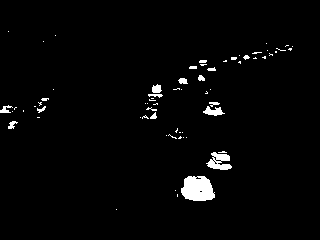
\includegraphics[width=0.3\columnwidth]{bgs_frame/ViBE/mask}


  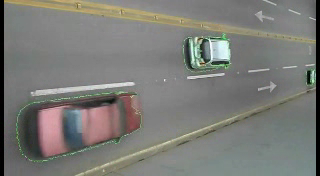
\includegraphics[width=0.3\columnwidth]{bgs_video/input}
  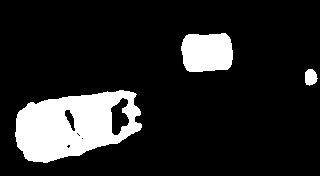
\includegraphics[width=0.3\columnwidth]{bgs_video/MultiLayerBGS/mask}
  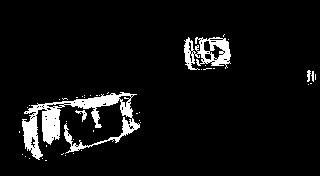
\includegraphics[width=0.3\columnwidth]{bgs_video/MixtureOfGaussianV1BGS/mask}
  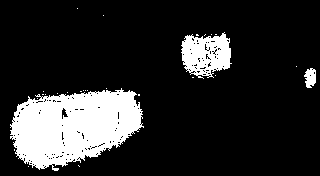
\includegraphics[width=0.3\columnwidth]{bgs_video/LBAdaptiveSOM/mask}
  
\includegraphics[width=0.3\columnwidth]{bgs_video/DPWrenGABGS/mask}
  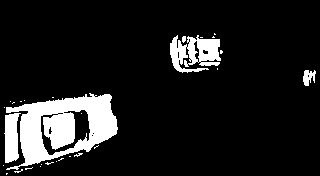
\includegraphics[width=0.3\columnwidth]{bgs_video/ViBE/mask}

  \caption{Exemplary frames of results obtained from background subtraction algorithms. Every 2 rows: Input frame, foreground mask obtained by MultiLayerBGS, MixtureOfGaussianV1BGS, LBAdaptiveSOM, DPWrenGABGS and ViBE algorithms.}
  \label{Figure:bgs_frame}
\end{figure}

%{\color{red}Background truth, how to tell best masks?}

The better the \moda{masks match} the moving object, the better the \moda{algorithm} is. It can be seen from \fref{Figure:bgs_frame} that MultiLayerBGS gave \mdc{fewer} holes in the foreground masks, LBAdaptiveSOM had large environment noises, MixtureOfGaussianV1BGS and DPWrenGABGS both produced a large hole in the masks from the second sample dataset. There are some false positions in the foreground mask obtained by ViBE from the first dataset, because the dataset was too short, \moda{so that} the ViBE algorithm \mdc{was} not fully learnt the background model yet. However the masks it computed were still close to the input frame, especially from the second dataset.

\section{Object tracking algorithms}

%Connected component analysis or blob detection (\sref{blob}) and movement tracking (\sref{bg:tracking}) algorithms were not implemented yet.

%A suitable camera module need to be ordered and interfaced afterwards, then implement automatic feedback control of frame rate, cropping and down sampling.

\subsection{Connected component analysis}

Connected component analysis was done as shown \mdc{in} \fref{imp:cca}. The baseline highway sample dataset from CDNET \cite{goyette2012changedetection} was used, it has 1700 frames, 30 frames per second and the resolution is $320 \times 240$. The ViBE background subtraction algorithm was used to extract foreground masks as shown \mdc{in} \fref{imp:cca:mask}, for connected component analysis algorithm to evaluate. OpenCV's find contours \modc{function was} used to extract the blobs. However, in order for it to work properly, the masks need to be cleaned up first. This was done by applying a find contours function first, filtering out small contours that are mostly likely noises, then redraw the contours. That may still \mdc{leave} unclosed holes, therefore a Morphology transformation \cite{serra1982image} was applied afterwards to close those holes. \fref{imp:cca:mask2} shows the mask been cleaned up. Finally, apply the find contours function to the enhanced foreground mask, results in numbers of contours, outlined on the input frame shown \mdc{in} \fref{imp:cca:drawing}.

\begin{figure}[htb]
  \centering
  \subfigure [] {
    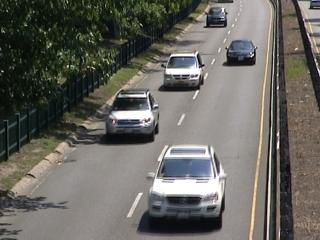
\includegraphics[width=0.4\columnwidth]{contours/input}
    \label{imp:cca:input}
  }
  \subfigure [] {
    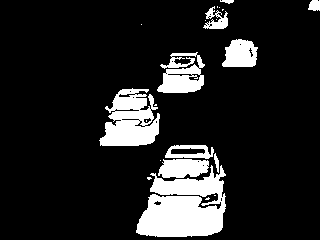
\includegraphics[width=0.4\columnwidth]{contours/mask}
    \label{imp:cca:mask}
  }
  \subfigure [] {
    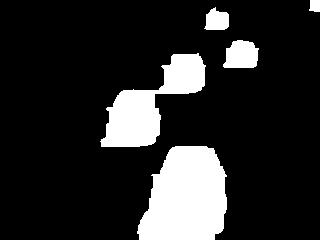
\includegraphics[width=0.4\columnwidth]{contours/img_mask}
    \label{imp:cca:mask2}
  }
  \subfigure [] {
    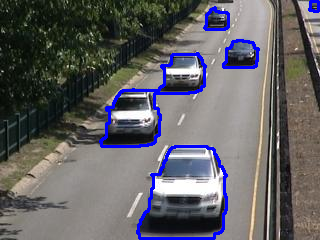
\includegraphics[width=0.4\columnwidth]{contours/drawing}
    \label{imp:cca:drawing}
  }
  \caption{Contours extracted from foreground masks. \subref{imp:cca:input} input frame, \subref{imp:cca:mask} foreground mask extracted by ViBE, \subref{imp:cca:mask2} enhanced foreground mask, \subref{imp:cca:drawing} contours (blobs) extracted}
  \label{imp:cca}
\end{figure}

%\subsection{Continuously Adaptive Meanshift}

\subsection{Optical flow}

\fref{imp:of} shows exemplary sparse set optical flow tracking result between 2 frames. The frames were taken from the baseline highway dataset from CDNET \cite{goyette2012changedetection}, but are 8 frames apart, in order to investigate how well the optical flow algorithm works when \modc{objects travel} too fast, \modc{move} a long distance between adjacent frames.

\begin{figure}[htb]
  \centering
  \subfigure [] {
    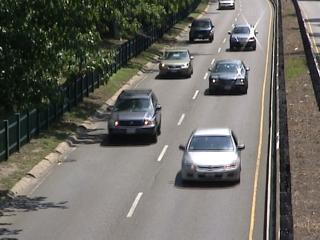
\includegraphics[width=0.3\columnwidth]{optical/between/prev}
    \label{imp:of:prev}
  }
  \iffalse
  \subfigure [] {
    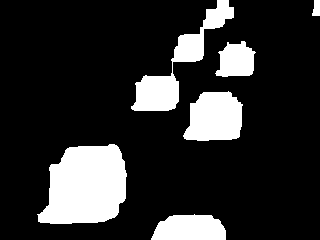
\includegraphics[width=0.3\columnwidth]{optical/between/prev_mask2}
    \label{imp:of:prev_mask}
  }
  \fi
  \subfigure [] {
    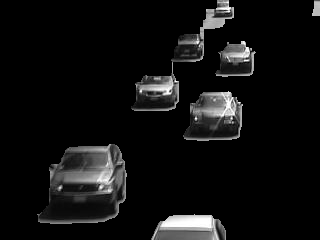
\includegraphics[width=0.3\columnwidth]{optical/between/prev_input_of}
    \label{imp:of:prev_input_of}
  }
  \subfigure [] {
    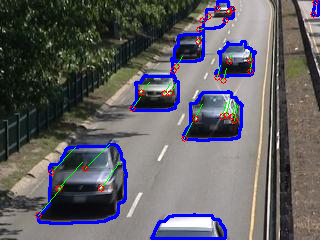
\includegraphics[width=0.3\columnwidth]{optical/between/prev_drawing}
    \label{imp:of:prev_drawing}
  }
  \subfigure [] {
    \includegraphics[width=0.3\columnwidth]{optical/between/next}
    \label{imp:of:next}
  }
  \subfigure [] {
    \includegraphics[width=0.3\columnwidth]{optical/between/next_input_of}
    \label{imp:of:next_input_of}
  }
  \subfigure [] {
    \includegraphics[width=0.3\columnwidth]{optical/between/next_drawing}
    \label{imp:of:next_drawing}
  }
  \caption{Sparse set optical flow tracking between 2 frames. \subref{imp:of:prev} previous frame, \subref{imp:of:prev_input_of} masked previous frame, \subref{imp:of:prev_drawing} optical tracking result at the previous frame, \subref{imp:of:next} next frame, \subref{imp:of:next_input_of} masked next frame, \subref{imp:of:next_drawing} optical flow tracking result at the next frame. {\color{red}Red circles}: Destinations of feature points generated from previous frame; {\color{dkgreen}Green lines}: Movements of the feature points; {\color{blue}Blue outline}: Object blobs extracted from foreground mask.}
  \label{imp:of}
\end{figure}

The feature points were taken from corner points along the edges of contours extracted by background subtraction algorithm. The input frames were also masked by the foreground masks as shown \mdc{in} \fref{imp:of:prev_input_of} and \fref{imp:of:next_input_of} to reduce possible distractions to the algorithm.

However, sometimes the optical flow algorithm may \mdc{give} incorrect tracking results, for example the 2 frames shown in \fref{imp:of:error}. To filtering out those occasions, it is necessary to estimate the maximum possible velocity of objects moving in the scene.

\begin{figure}[htb]
  \centering
  \subfigure [] {
    \includegraphics[width=0.45\columnwidth]{optical/error/000170_drawing}
    \label{imp:of:error:1}
  }
  \subfigure [] {
    \includegraphics[width=0.45\columnwidth]{optical/error/000171_drawing}
    \label{imp:of:error:2}
  }
  \caption{Situation when optical flow gives unrealistic results for 2 frames from CDNET baseline PETS2006 dataset. {\color{dkgreen}Green lines}: Movements of the feature points; {\color{blue}Blue outline}: Object blobs extracted from foreground mask.}
  \label{imp:of:error}
\end{figure}

By relating the destination of movements of feature points from blobs in previous frame to blobs detected in the next frame, the blobs can be tracked between frames. However this is not required for \modb{obtaining} the \modb{highest} speed of \modb{objects moving between frames, which is the input the adaptive operation depends on. Implementing} this would \modb{also} require lots of efforts for statistic computation to filtering out incorrect tracking results, point in polygon testing \modb{algorithm} and blob management, therefore was considered as further work.

\section{\modc{Adaptive \modb{energy} saving operation}}

Adaptive energy saving operation was done by varying input video stream frame rate based on object tracking results, a feedback loop as previous illustrated in the system block diagram (\fref{block}).

\subsection{Parameter metrics}

For it to work optimistically in a particular scenario, a few parameter metrics are required, listed in \tref{imp:ada:par}.

\begin{table}[H]
  \centering
  \begin{tabular}{cc}
  \toprule
  \textbf{Parameter metric} \\
  \midrule
  Maximum possible object moving speed. \\
  Typical object sizes. \\
  Typical distances between objects. \\
  Active area masks. \\
  Minimum acceptable frame rate. \\
  Maximum possible frame rate. \\
  \bottomrule
  \end{tabular}
  \caption{Parameter metrics required for adaptive energy saving operation}
  \label{imp:ada:par}
\end{table}

The basic one is the maximum possible moving speed of any objects and parts of objects in the scenario. It is used to determine all other parameters.

Typical object sizes, distances between objects and active area masks are used to optimise foreground mask filtering, so that noises and movements caused by other unrelated objects and noises can be filtered out as much as possible. They are irrelevant to the optical flow tracking algorithm, because the algorithm is tracking feature points around blobs not shapes of blobs.

The minimum frame rate is determined as shown by \eref{f_min}, so that movement of any object will not overtake the tracking window, therefore most likely keep been tracked. It is also limited by minimum response rate required in an application.

\begin{equation}
	f_{min} = \frac{\text{Maximum object speed}}{\text{Optical flow optimum tracking length}}
	\label{f_min}
\end{equation}

The maximum frame rate is only limited by algorithm computation speed and hardware limitations.

\subsection{Frame rate adaptation}

Having calculated the maximum movement distance of feature points between adjacent frames, the frame rate is then calculated as \eref{f_rate}. The frame interval will be adjusted according to this by the main thread.

\begin{equation}
	f = \frac{\text{Maximum movement distance}}{\text{Optical flow optimum tracking length} \times \text{Time between frames}}
	\label{f_rate}
\end{equation}

{\color{red}Implementation? BOOM}
%\section{Video stream dataset}

\chapter{Analysis} \label{Chapter:Analysis}

\section{Camera frame rate calculation}

\todo{BOOM}

\section{Power consumption modelling}

Power consumption modelling was done by measuring the average power consumption of the algorithm running under different frame rates, with frames captured from the camera module.

\todo{BOOM}

\section{Power consumption reduction analysis}

Power consumption reduction was analysed using the video datasets from CDNET, to keep input video stream consistent. However, because the frame images inside the datasets are discrete in time, the frame rate cannot be changed in great precision, results in a rough estimation of the actual performance.

Firstly, some properties of the dataset under test need to be determined, such as maximum object moving speed and minimum FPS required. This is done by evaluate the dataset without adaptive operation. During the process, the maximum distances objects moved between each frame intervals were recorded. The top $5 \%$ of the distances that are most likely due to errors were removed. \fref{ana:ada} shows the distribution of maximum moving distances after filtering in a dataset. The maximum of those value was considered as the maximum speed an object may travel in the dataset. According to the formulae described in section \ref{imp:ada:metric}, the minimum FPS requirement was then calculated. The optical flow tracking window was set to 32 pixels, as a result most minimum FPS requirements calculated were under 1 FPS. For a faster response time, the minimum FPS was set to 2 FPS.

\begin{figure}[htb]
  \centering
  \subfigure [Absolute maximum distances objects travelled between frames] {
    \includegraphics[width=0.45\columnwidth]{ana_ada_xy}
    \label{ana:ada:xy}
  }
  \subfigure [Histogram distribution of maximum distances] {
    \includegraphics[width=0.45\columnwidth]{ana_ada_histo}
    \label{ana:ada:histo}
  }
  \caption{Filtered distributions from CDNET highway dataset.}
  \label{ana:ada}
\end{figure}

By applying the power consumption model, the actual power consumption can be estimated.

\begin{figure}[htb]
  \centering
  \includegraphics[width=\columnwidth]{ana_summary}
  \caption{Summary of evaluated CDNET datasets.}
  \label{ana:summary}
\end{figure}

\todo{BOOM}

\chapter{Conclusion} \label{Chapter:Conclusion}

\section{Achievements}

The camera driver was successfully developed, and was able to configure the camera sensor, capture still images and video streams.

Several object detection and tracking algorithms were investigated.

An application running adaptive object tracking algorithms was developed. The algorithms can run at 30 FPS as in specification. The effect of adaptive operation was investigated. All objects in the sample datasets get tracked regardless of whether the adaptive operation is applied or not.

By applying adaptive operation, power consumption reduction estimation of $19 \%$ was achieved for varies video surveillance datasets. It was only $19 \%$, due to the high standby power consumption of the embedded development board. The adaptive operation still has an effect on power consumption, but was not very significant compare to standby power consumption.

%\todo{Power saving achieved.
%Compare back to aims, specifications. (Why didn't?)}

\section{Constraints}

The algorithms used can only run at around 30 FPS maximum with $320 \times 240$ resolution. Objects moves faster than this, such as a basket ball may need a faster frame rate to be tracked. The maximum speed is also highly depending on the object to camera distance.

The algorithms implemented can only works with a steady background, limiting the application area to still camera application such as video surveillance.

\section{Further work}

\subsection{Camera driver}

The camera driver in collaboration with NVIDIA's MIPI-CSI driver is not stable enough. In case the application that are using the camera being forced stopped by the user or due to a programming bug, the drivers may crash the kernel due to lost synchronisation. This need further investigation.

When a buffer been marked as filled by the MIPI-CSI driver, it is actually still receiving data from the camera. Possible reasons are losing or misinterpreting synchronisation packets, camera configuration problem and bugs in MIPI-CSI driver implementation. A workaround was used, by receiving 2 filled buffers from the driver, then use the first one as valid data. However, this workaround gives 2 frames latency regardless of frame rate. This need further investigation.

The driver interface for controlling the frame rate, configuring exposure settings etc. need to be completed and standardised.

The Tegra K1 CPU has a built-in ISP that can convert Bayer pattern to standard RGB format without using CPU or GPU time. However, the documentation of this feature is confidential. The NVIDIA's video interface driver that are using this ISP is also undocumented in public domain. Power consumption may be reduced further if the ISP can be used.

\subsection{Application}

The application structure may be made more efficient.

The application can be a lot easier to use and configure with a better user interface.

Transmission of video stream and tracking results through network for Internet-of-Things applications may be useful to implement.

\subsection{Algorithms}

Further optimisations to the algorithms are possible. More efficient implementations that supports better resolution and faster frame rate are desired.

Blob tracking algorithm based on optical flow tracking results may be implemented.

More algorithms may be investigated. Especially algorithms that handle background movement, which are very useful in automotive applications.

\section{Evaluation}

During implementation, I found that I spent a lot time trying to stabilise the camera driver to prefect. That is not the main goal of the project, the camera driver was actually usable for algorithm analysis. Therefore I chose to accept the problems with the drivers, and moved the diagnosis works to further work.

%\todo{Difficulties, solutions etc.}

\chapter{Project management}

\section{Risk management}

\begin{table}[!htb]
  \centering
  \begin{tabular}{|p{0.16\columnwidth}|c|c|p{0.42\columnwidth}|}
  \hline
  \textbf{Risk (event)} & \textbf{Likelihood} & \textbf{Impact} & \textbf{Action} \\ \hline
  Camera module failure & Low & High & Buy redundant camera modules. \\ \hline
  Jetson board failure & Low & High & Find another one, or find alternative ways to continue the project. \\ \hline
  Test facilities not available & Low & Medium & Check in advance. \\ \hline
  ECS file storage server is slow & Medium & Medium & Use my own laptop. \\ \hline
  Supervisor is away at meeting & High & Low & Read literatures, continue implementations. \\ \hline
  Unexpected accident or illness & Low & High & Try to avoid. Have multiple backups. \\ \hline
  Unable to implement camera driver & Medium & High & Find easy alternatives, or read frames from video files. \\ \hline
  Unable to implement some algorithms & Medium & High & Find easy alternatives. \\ \hline
  \end{tabular}
  \caption{Risk assessment}
  \label{man:risk}
\end{table}

\subsection{Board failure}

During the second semester, the Jetson board accidentally failed on 3rd, Match. I was probing a current sensor resistor on the board, then unintentionally short circuited the 12V power rail to the 3.3V power rail. Although the CPU, GPU cores and some peripheral interfaces survived, two of the power rails were still in short circuit condition and cannot be easily diagnosed. As a result, USB, Ethernet and HDMI interfaces were not functioning. The board can only be controlled through a UART interface, with a voltage level converter chip. Power consumption analysis would also be affected by the two short circuited power rails.

I quickly transferred the algorithm development to a general purpose computer to continue working on it. This could be done only because all the source codes were regularly backed up on the git server. Having recognised that the board is only essential for power consumption modelling, reasonable results were still possible even without the board. The algorithms can run on a general computer, most analyses are still possible. Finally, after some negotiation with my supervisor, another board was available for use, the development was then transferred to the new board.

\section{Time management}

The topic of project changed once during week 7 in semester 1. The previous topic (\aref{Appendix:brief_prev}) was about reducing power consumption for algorithms that are utilising General Purpose GPU (GPGPU) technique, by adaptively controlling calculation precision. The NVIDIA Jetson TK1 development platform was decided to be used in this project. However, after investigated into the topic and experimented with some algorithms, the purposed precision control did not contribute significant impact on computation quality. Not much power saving would be possible to be made.

Therefore, I decided to change the project topic. The current project topic (\aref{Appendix:brief}) was quickly determined. The same hardware platform was still used, so that the time invested in the previous project was not wasted. Therefore, I was able to quickly catch up with the progress.

The Gantt chart was also changed due to project topic changing, as shown in \fref{gantt_prev} and \fref{gantt_rev}. The time invested for previous project topic was treated as background reading. \fref{gantt} shows the actual time spend on each of the items.

\begin{figure}[H]
  \centering
  \includegraphics[width=\columnwidth]{Gantt_previous}
  \caption{Previous Gantt chart}
  \label{gantt_prev}
\end{figure}

\begin{figure}[H]
  \centering
  \includegraphics[width=\columnwidth]{Gantt_interim}
  \caption{Revised Gantt chart}
  \label{gantt_rev}
\end{figure}

\begin{figure}[H]
  \centering
  \includegraphics[width=\columnwidth]{Gantt}
  \caption{Actual time usage}
  \label{gantt}
\end{figure}

\section{Backing up}

%Source code management.
%Documents and materials.

The git version control system \cite{git} was used in this project. It has the feature that allows multiple users collaborate on the same repository. However, this is an individual project, git was used purely for backing up source code version history and synchronisation between multiple devices. Well-known git hosting website GitHub \cite{github} and university's SourceKettle server \cite{sourcekettle} were used for multiple backups.

All documents, background literals and materials used by the project were backed up using Microsoft's OneDrive service.

%\section{Remaining work}

%\begin{itemize}
%  \item Movement tracking based on blob detection (Section \ref{bg:tracking}, \ref{impl:tracking}).
%  \item A camera module need to be ordered and interfaced.
%  \item Automatic frame rate reduction based on tracking result.
%  \item Hardware downsampling and cropping based on ROI.
%  \item If time allows, energy-efficient object recognition may be implemented.
%\end{itemize}


%\appendix

\begin{appendices}
\titleformat{\chapter}[hang]{\Large\bfseries}{\chaptertitlename\ \thechapter}{0.75cm}{\Large\bfseries}
%% ----------------------------------------------------------------
%% Appendix:brief
%% ----------------------------------------------------------------
\chapter{Agreed project brief}
\label{Appendix:brief}

\begin{figure}
\centering
\includepdf[pages={1}, offset=0 -2cm, trim={0, 0, 0, 0}, clip]{inc/Brief.pdf}
\end{figure}

\clearpage

%% ----------------------------------------------------------------
%% Appendix:brief_prev
%% ----------------------------------------------------------------
\chapter{Previous project brief}
\label{Appendix:brief_prev}

\begin{figure}
\centering
\includepdf[pages={1}, offset=0 -2cm, trim={0, 0, 0, 0}, clip]{inc/Brief_previous.pdf}
\end{figure}

\clearpage

\chapter{Costs} \label{Appendix:Costs}

Bill of materials

\clearpage

\chapter{Contents of design archive} \label{Appendix:Archive}

Contents of design archive

\clearpage

%%% ----------------------------------------------------------------
%% Appendix:gantt
%% ----------------------------------------------------------------
\chapter{Porject Gantt charts}
\label{Appendix:gantt}

\begin{figure}[H]
  \centering
  \subfigure [{Previous Gantt chart}] {
    \includegraphics[page=1, trim={1cm, 5cm, 4cm, 1cm}, clip, width=\columnwidth]{inc/Gantt_previous.pdf}
  }
  \subfigure [{Current Gantt chart}] {
    \includegraphics[page=1, trim={1cm, 5cm, 4cm, 1cm}, clip, width=\columnwidth]{inc/Gantt.pdf}
  }
\end{figure}

\clearpage

\end{appendices}

\backmatter
\bibliography{Reference}
\end{document}
%% ----------------------------------------------------------------
